%% ---------------------------------------------------------------------------
%% Copyright 2015 Matthias Vogelgesang and the LaTeX community. A full list of
%% contributors can be found at
%%
%%     https://github.com/matze/mtheme/graphs/contributors
%%
%% and the original template was based on the HSRM theme by Benjamin Weiss.
%%
%% This work is licensed under a Creative Commons Attribution-ShareAlike 4.0
%% International License (https://creativecommons.org/licenses/by-sa/4.0/).
%% ---------------------------------------------------------------------------

\documentclass[10pt]{beamer}

\usetheme{metropolis}
\usepackage{appendixnumberbeamer}

\usepackage{booktabs}
\usepackage[scale=2]{ccicons}
%----------------------------
\newcommand\alertitem[1]{\alert<+>{\item {#1}}}
\usepackage[lined,ruled,vlined,commentsnumbered]{algorithm2e}

\newcommand*{\MG}{\VarCal{M}}  
%To draw pictures
\usepackage{pgf}
\usetikzlibrary{arrows,automata}
\usetikzlibrary{positioning}
\usetikzlibrary{calc}
\usetikzlibrary{shapes.geometric}
\usetikzlibrary{arrows.meta}
\usetikzlibrary{decorations.pathmorphing}

\usepackage{amsthm}
\theoremstyle{plain}
\newtheorem{thm}{Theorem}
\newtheorem{lem}{Lemma}

\theoremstyle{definition}
\newtheorem{defn}{Definition}
\newtheorem{observation}{Observation}
\newcommand{\Tau}{\mathrm{T}}
\newcommand*{\Secref}[1]{Section ~{#1}}

\newcommand*{\withbot}[1]{{#1}_\bot}
\newcommand*{\Nbot}{\withbot{N}}
\newcommand*{\Pbot}{\withbot{P_0}}

\newcommand*{\Var}[1]{\ensuremath{\mathit{#1}}}
\newcommand*{\Sec}[1]{Sec.~\ref{#1}}
\newcommand*{\Alg}[1]{Algorithm~\ref{#1}}
\newcommand*{\Fig}[2][]{Fig.~\ref{#2}{#1}}

\newcommand*{\Unseen}{\Var{Unseen}}
\newcommand*{\Seen}{\Var{Seen}}
\newcommand*{\Visited}{\Var{Visited}}

\newcommand*{\Active}{\Var{active}}
\newcommand*{\Born}{\Var{born}}
\newcommand*{\Needed}{\Var{needed}}
\newcommand*{\Origins}{\Var{origins}}

\newcommand*{\RangeOfReset}{\Var{range}\_\Var{of}\_\Var{reset}}
\newcommand*{\Range}{\Var{range}}
\newcommand*{\Ranges}{\Var{Ranges}}
\newcommand*{\RangeOfClock}{\Var{range}\_\Var{of}\_\Var{clock}}
\newcommand*{\PartitionIntoASetOfGroups}
{\Var{partition}-\Var{into}-\Var{a}-\Var{set}-\Var{of}-\Var{groups}}

\newcommand*{\Ind}{\hspace{1em}}

\newcommand*{\Rel}[1]{\ensuremath{\Var{rel}_{#1}}}   % relation of being related
\newcommand*{\RelClosure}[1]{\ensuremath{\Rel{#1}^*}}       % and its closure
\newcommand*{\Relate}[2]{\ensuremath{\Var{Rel}(#1, #2)}}

%----------------------------
\usepackage{pgfplots}
\usepgfplotslibrary{dateplot}
\usepackage{adjustbox}
\usepackage{xspace}
\newcommand{\themename}{\textbf{\textsc{metropolis}}\xspace}

\title{From Scenarios to Optimally Allocated Timed Automata}
%\subtitle{A modern beamer theme}
\date{\today}
\author{Sandeep Vuppula}
\institute{University of Minnesota Duluth}
% \titlegraphic{\hfill\includegraphics[height=1.5cm]{logo.pdf}}

\begin{document}

\maketitle

\begin{frame}{Table of contents}
  \setbeamertemplate{section in toc}[sections numbered]
  \tableofcontents[hideallsubsections]
\end{frame}

\begin{frame}{Objectives of the Research}
	Our main focus of the research is:
	\begin{enumerate}
		\item	To synthesize a timed automaton from a set of scenarios, and
		\item	To optimally allocate clocks in the constructed timed automaton.
	\end{enumerate}
\end{frame}

\section{Background}

%\begin{frame}{Real-time systems}
%	\begin{itemize}
%		\item A real-time system takes input from its surrounding environment and produces results within a stipulated amount of time.
%		\item In the real world, the behaviour of almost every system changes according to time.
%		\item We can model such real time systems with the help of timed automata.
%	\end{itemize}
%\end{frame}

\begin{frame}{Modeling Time}
	There are three approaches for modeling time:
	\begin{itemize}		
		\item \underline{Discrete time model}: Time is considered as discrete and monotonically increasing sequence of integers. Limits the preciseness: in real-time systems, the events do not occur at integer times.
		%\pause
		\item \underline{Fictitious-clock model}: It is similar to that of discrete time model except that it assumes sequence of times to be non decreasing integers. Limits accuracy, as the exact time values at which the events occur are not considered. 
		%\pause
		\item \underline{Dense time model}: In this model, the domain of time is a set of real numbers, and the sequence of times increase monotonically without any limit. %considered as a dense set and the time of occurrences of events as real numbers, which increase monotonically without any limit. Difficulty in transforming dense time traces into formal languages.
	\end{itemize}
\end{frame}


\begin{frame}{Timed Automata}
	\begin{itemize}
		\item A timed automaton is a finite state automaton extended with a finite set of real-valued clocks. 
		\item Upon an input, the selection of next state is based not only on the input symbol but also on the time of the current symbol with respect to the formerly read symbols. 
	\end{itemize}
	%\pause
%	\textbf{Example:} Consider a simple timed automaton in Figure \ref{fig:fig1}. This automaton accepts an input sequence `a' followed by `b' such that, there is 2 units of time difference between any two consecutive a's and b's.
%	
%	\begin{figure}
%		\centering
%		\includegraphics[width=0.5\linewidth]{"fig1"}
%		\caption{A simple timed automaton}
%		\label{fig:fig1}
%	\end{figure}
\end{frame}

\begin{frame}{%What is timed automata?\\
	A simple light control}
\begin{figure}[!t]
	\begin{center}
		%\begin{minipage}[b]{0.3\textwidth}
		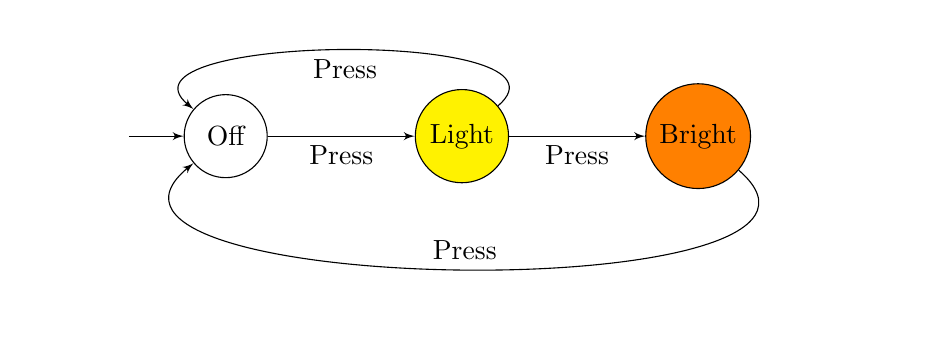
\begin{tikzpicture}
		
		\tikzset{vertex/.style = {shape=circle,draw,minimum size=3em}}
		\tikzset{vertex2/.style = {shape=circle,draw=none,minimum size=1.5em}}
		\tikzset{edge/.style = {->,> = latex'}}
		% vertices
		\node[vertex] (b) at  (0,0) {Off};
		\node[vertex, fill = yellow] (c) at  (3, 0) {Light};
		\node[vertex, fill = orange] (d) at  (6, 0) {Bright};
		
		\node[vertex2] (a) at  (-1.5,0) {};
		
		%edges
		\draw[edge] (a) to (b);        
		
		\draw[edge] (b) to node[below]{Press}  (c);
		
		\draw[edge] (c) to node[below]{Press} (d) ;
		
		\draw[edge] (d) to [bend left = 500 pt] node[above]{Press}  (b);
		
		\draw[edge] (c) to [bend right = 500 pt] node[below]{Press} (b);
		
		
		\end{tikzpicture}
		%\caption{A timed automaton (in \OurLargerClass)}\label{incorrect}
		% \end{minipage}
		
	\end{center}
\end{figure}
Desired behavior: if Press occurs twice {\textcolor{red} {quickly}} then the light gets brighter, otherwise the light turns off.
\end{frame}

%%%%%%%%%%%%%%%%%%%%

\begin{frame}{A simple light control}
\begin{figure}[!t]
\begin{center}
	%\begin{minipage}[b]{0.3\textwidth}
	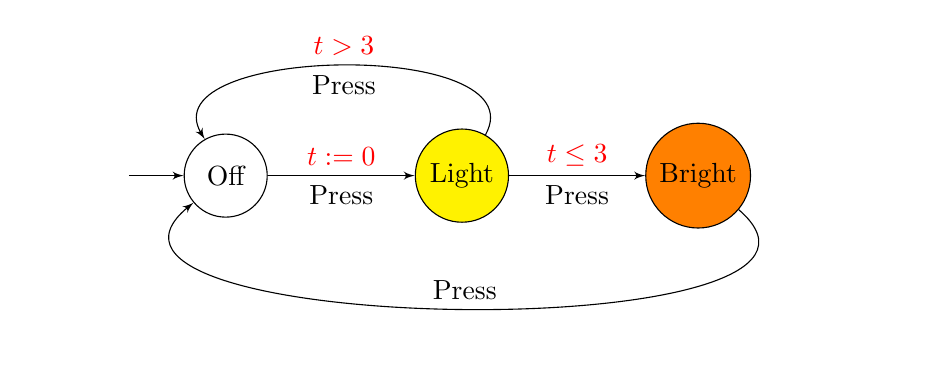
\begin{tikzpicture}
	\tikzset{vertex/.style = {shape=circle,draw,minimum size=3em}}
	\tikzset{vertex2/.style = {shape=circle,draw=none,minimum size=1.5em}}
	\tikzset{edge/.style = {->,> = latex'}}
	% vertices
	\node[vertex] (b) at  (0,0) {Off};
	\node[vertex, fill = yellow] (c) at  (3, 0) {Light};
	\node[vertex, fill = orange] (d) at  (6, 0) {Bright};
	
	\node[vertex2] (a) at  (-1.5,0) {};
	
	%edges
	\draw[edge] (a) to (b);        
	
	\draw[edge] (b) to node[above]{\textcolor{red}{$t := 0$}} node[below]{Press}  (c);
	
	\draw[edge] (c) to node[above]{\textcolor{red}{$t\leq 3$}} node[below]{Press} (d);
	
	\draw[edge] (d) to [bend left = 500 pt] node[above]{Press}  (b);
	
	\draw[edge] (c) to [bend left = 600 pt] node[above]{\textcolor{red}{$t > 3$}} node[below]{Press} (b);
	
	%\node[draw,align=left] at (6,1) {some text\\ spanning three lines\\ with manual line breaks};
	
	%\draw decorate {(0,0) -- (2,2)};
	
	%\node[decorate,draw,inner sep=0.5cm,fill=yellow,circle] (a) at (2,0) {};
	
	\end{tikzpicture}
	%\caption{A timed automaton (in \OurLargerClass)}\label{incorrect}
	% \end{minipage}
	
\end{center}
\end{figure}
Solution: finite state machines augmented with real-valued clocks.%$c$ is a real-valued clock
\end{frame}

%%%%%%%%%%%%%%%%%%%%%%%%%%%%


\begin{frame}{Timed automata}
	\begin{figure}[!t]
	\begin{center}
		%\begin{minipage}[b]{0.3\textwidth}
		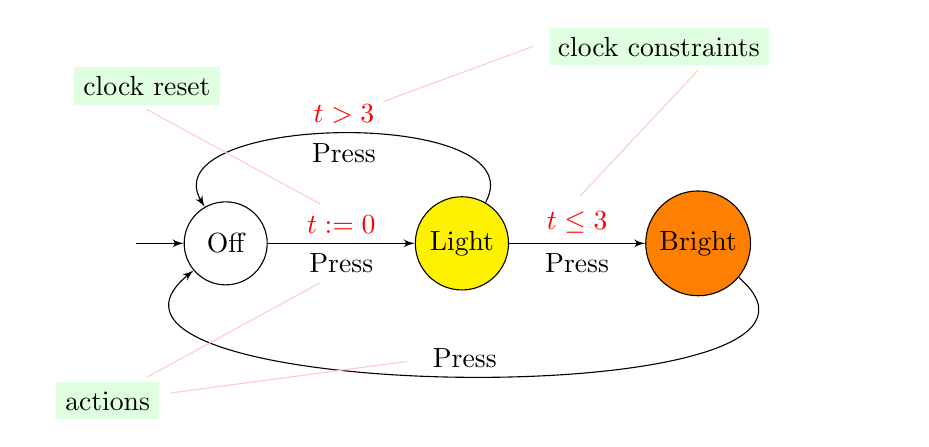
\begin{tikzpicture}
		\tikzset{vertex/.style = {shape=circle,draw,minimum size=3em}}
		\tikzset{vertex2/.style = {shape=circle,draw=none,minimum size=2em}}
		\tikzset{edge/.style = {->,> = latex'}}
		% vertices
		\node[vertex] (b) at  (0,0) {Off};
		\node[vertex, fill = yellow] (c) at  (3, 0) {Light};
		\node[vertex, fill = orange] (d) at  (6, 0) {Bright};
		
		\node[vertex2] (a) at  (-1.5,0) {};
		
		%edges
		\draw[edge] (a) to (b);        
		
		\draw[edge] (b) to node[above]{\textcolor{red}{$t := 0$}} node[below]{Press}  (c);
		
		\draw[edge] (c) to node[above]{\textcolor{red}{$t\leq 3$}} node[below]{Press} (d);
		
		\draw[edge] (d) to [bend left = 500 pt] node[above]{Press}  (b);
		
		\draw[edge] (c) to [bend left = 600 pt] node[above]{\textcolor{red}{$t > 3$}} node[below]{Press} (b);
		
		\node[align=left, fill = green!12] at (5.5,2.5) {clock constraints};
		\node[align=left, fill = green!12] at (-1,2) {clock reset};
		\node[align=left, fill = green!12] at (-1.5,-2) {actions};
		
		\draw[color = red!20] decorate {(4.5,0.6) -- (6,2.2)};
		\draw[color = red!20] decorate {(2,1.8) -- (3.9,2.5)};
		\draw[color = red!20] decorate {(1.2,0.5) -- (-1,1.7)};
		\draw[color = red!20] decorate {(1.2,-0.5) -- (-1,-1.7)};
		\draw[color = red!20] decorate {(2.3,-1.5) -- (-0.7,-1.9)};
		
		%\node[decorate,draw,inner sep=0.5cm,fill=yellow,circle] (a) at (2,0) {};
		
		\end{tikzpicture}
		%\caption{A timed automaton (in \OurLargerClass)}\label{incorrect}
		% \end{minipage}
	
	\end{center}
	\end{figure}
%Solution: finite state machines augmented with real-valued clocks.%$c$ is a real-valued clock
\end{frame}

%%%%%%%%%%%%%%%%%%%%%

\begin{frame}{Timed Automata: syntax}
	\begin{block}{}
		For a set $V$ of clock variables:
		\begin{itemize}
		\item
		the set $\Phi(V)$ includes \emph{clock constraints} of the form $t\sim a$, where 
			\begin{itemize}
				\item
				$t\in V$, 
				\item
				$\sim\in\{\leq, \geq, <, >, =\}$, 
				\item
				$a$ is a constant in the set of rational numbers, $\mathbb{Q}$.
			\end{itemize}
		\end{itemize}
	\end{block}
	A \emph{timed automaton} is a tuple ${\cal A} = \langle \Sigma, Q, Q_0, V, E \rangle$, where
	\begin{itemize}
		\item $\Sigma$  is a finite set of labels/actions (alphabet)
		\item $Q$ is a finite set of states
		\item $Q_0 \subseteq Q$ is a set of initial states
		\item $V$ is a finite set of clocks
		\item $E \subseteq Q \times Q \times \Sigma \times 2^{V} \times 2^{\Phi(V)}$ is a finite set of edges of the form $(q, q^\prime, \sigma, \lambda, \phi)$, where 
			\begin{itemize}
			\item
			$\lambda \subseteq V$ is the clocks to be reset with this transition, 
			\item
			$\phi$ is a set of clock constraints over $V$.
			\end{itemize}
	\end{itemize}
\end{frame}

%%%%%%%%%%%%%%%%%%%%%%%%%%%%%%

\begin{frame}{Timed automata}
	\begin{figure}[!t]
	\begin{center}
%\begin{minipage}[b]{0.3\textwidth}
		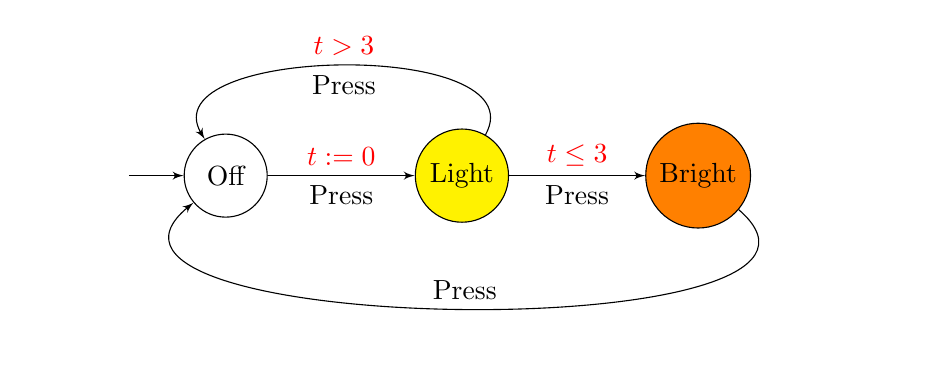
\begin{tikzpicture}
		\tikzset{vertex/.style = {shape=circle,draw,minimum size=3em}}
		\tikzset{vertex2/.style = {shape=circle,draw=none,minimum size=1.5em}}
		\tikzset{edge/.style = {->,> = latex'}}
		% vertices
		\node[vertex] (b) at  (0,0) {Off};
		\node[vertex, fill = yellow] (c) at  (3, 0) {Light};
		\node[vertex, fill = orange] (d) at  (6, 0) {Bright};
		
		\node[vertex2] (a) at  (-1.5,0) {};
		
		%edges
		\draw[edge] (a) to (b);        
		
		\draw[edge] (b) to node[above]{\textcolor{red}{$t := 0$}} node[below]{Press}  (c);
		
		\draw[edge] (c) to node[above]{\textcolor{red}{$t\leq 3$}} node[below]{Press} (d);
		
		\draw[edge] (d) to [bend left = 500 pt] node[above]{Press}  (b);
		
		\draw[edge] (c) to [bend left = 600 pt] node[above]{\textcolor{red}{$t > 3$}} node[below]{Press} (b);
		
		\end{tikzpicture}
		%\caption{A timed automaton (in \OurLargerClass)}\label{incorrect}
		% \end{minipage}
		
	\end{center}
	\end{figure}
	The languge accepted by the automaton: \\
		\vdots
		$(press, 5) (press, 6.5) (press, 20) (press, 50) (press, 65) ...$
		$(press, 3) (press, 9) (press, 15) (press, 19) (press, 100) ...$\\
		\vdots
\end{frame}

\begin{frame}{Timed Automata: Undecidable Problem}
	\begin{itemize}
		\item The number of clocks in a given timed automaton has a direct impact on verification of the system.
		\item Given a timed automaton $\cal A$, the problem of deciding whether there exists another timed automaton $\cal B$ that accepts the same language as that of $\cal A$ but with fewer number of clocks is undecidable.
		
	\end{itemize}
	\vspace{0.5cm}
	
	%\pause
	%	\alert{	We formulate some criteria for a class of timed automata. Given a timed automaton that belongs to our class, we propose a method to optimally allocate clocks in that automaton.} %Given a timed automaton that belongs to our class, we use \emph{liveness analysis} of clocks to optimally allocate clocks.}
%	\alert{We propose a method to optimally allocate clocks in a timed automaton.}
\end{frame}

%\begin{frame}{Finite State Automata}
%	A finite state automaton (FSA) or a finite state machine (FSM) is an abstract machine which has a finite number of states. On an input, the machine changes from one state to another state.%: this is called a transition. %A FSA has a set of states, inputs, transitions, intial states and final states. 
%	
%	\begin{figure}
%	\begin{adjustbox}{max totalsize={.99\textwidth}{.8\textheight},center}
%		
%		\begin{tikzpicture}[->,>=stealth',shorten >=1pt,auto,node distance=2.5cm, semithick]
%		\tikzstyle{every state}=[draw,minimum size=3.5em]
%		
%		\node[initial,state]       (S1)                       {$Initial$};
%		\node[state]       (S2)    [right of=S1]      {$t_{found}$};
%		\node[state]       (S3)    [right of=S2]      {$i_{found}$};
%		\node[state]       (S4)    [right of=S3]      {$m_{found}$};
%		\node[state,accepting]       (S5)    [right of=S4]      {$success$};
%		\node[state]       (S6)    [below of=S3]      {$error$};
%		
%		
%		\path 	(S1)   edge          		node[anchor=south, above] {t}     (S2)
%		(S2)   edge                 node[anchor=south, above] {i}	  (S3)
%		(S3)   edge                 node[anchor=south, above] {m} 	  (S4)
%		(S4)   edge   				node[anchor=south, above] {e}     (S5)   
%		(S1)   edge          		node[sloped, above] {not\_t}     (S6)
%		(S2)   edge                 node[sloped, above] {not\_i}	  (S6)
%		(S3)   edge                 node[sloped, above] {not\_m} 	  (S6)
%		(S4)   edge   				node[sloped, above] {not\_e}     (S6)   
%		;
%		\end{tikzpicture}
%	\end{adjustbox}
%	\caption{Simple FSM parsing the string ``time"}
%	\label{fig:FSM}		
%	\end{figure}
%\end{frame}


\section{Motivation}

\begin{frame}{Motivation}
	\begin{itemize}
		\item Model-based design is a very effective method for designing real-time systems.
		\item Modeling a system formally can help us to understand the desired and undesired behaviours of the system.
%		\item In many real-time systems safety is critical.
		\item Building formal models for systems is challenging because of the lack of good formal requirements specifications.
	\end{itemize}	
\end{frame}

\begin{frame}{Motivation}
	\begin{itemize}
		\item	{To construct a formal model of a system, the following questions are to be answered first:
					\begin{enumerate}
						\item How the requirements should be expressed formally, and
						\item How the formal model of the system can be constructed from requirements.
					\end{enumerate}
				}
			%\pause
		\item {The formal model that we build is \alert{timed automata}.}
\end{itemize}
\end{frame}

\begin{frame}{Contribution 1}
%	Synthesizing timed automaton
	\begin{itemize}
		\item We use scenarios to build a formal model of a real-time system. %A scenario is a partial description of the behaviour of a system,
%		\item We propose Timed Event Sequences (TES) to formally represent the scenarios, and
		\item We use mode graphs to specify the legal events that can occur in the system.
	\end{itemize}
	%\pause
	\alert{We synthesize a \emph{minimal}, \emph{acyclic} and \emph{deterministic} timed automaton given a set of scenarios and a mode graph.}
\end{frame}

%\begin{frame}{Introduction}
%	Our timed automaton belongs to a class of timed automata that satisfies the following properties:
%	\begin{itemize} 
%		\item A clock $t_{j}$ can be reset only on the transitions emanating from a state labelled $j$ and,
%		\item A clock in a clock constraint on a transition $r$ from a state $q$ can only refer to a clock that has been reset on a transition leaving a state that dominates $q$. We call this \emph{dominance assumption}.
%	\end{itemize}
%\end{frame}

\begin{frame}{Contribution 2}
	\begin{itemize}
		\item We propose a method to optimally allocate clocks in a timed automaton.
		\item We perform liveness analysis of clocks in a timed automaton and use that information to minimize the number of clocks and optimally allocate them.
	\end{itemize}
\end{frame}

\section{Contributions}
\subsection{Synthesis of Timed Automata from Scenarios}

\begin{frame}{Synthesis of Timed Automata from Scenarios}
Our method of synthesizing a timed automaton model of a real-time system from scenarios involves two steps:
	\begin{enumerate}
		\item Constructing a time annotated graph from a set of scenarios, and
		\item Transforming this graph to the final timed automaton.
	\end{enumerate}
\end{frame}

\begin{frame}{%Synthesis of Timed Automata from Scenarios}
	Scenarios}
	\begin{itemize}
%		\item {Our approach for building a formal model is using scenarios.} 
		\item A scenario is a partial description of the behaviour of a system.
		\item A scenario not only describes the events, but also the timing relations among the events.
		\item A set of scenarios can capture the behaviour of a real-time system.
		
		%\pause
		\item We use \emph{mode graphs} to specify the legal events that can occur in the system.
		\item We propose Timed Event Sequences (TES) to describe the scenarios formally.
	\end{itemize}	
\end{frame}


\begin{frame}{Mode Graph}
A \emph{mode graph} is a deterministic state machine in which the states are called modes and the transitions triggered by the events in the system. \\
It is a tuple $\mathcal{M} = (M, m_0, m_f, \Sigma, T)$ where,
\begin{itemize}
	\item $M$ is a finite set of modes,
	\item $m_0$ is the initial mode, 
	\item $m_f$ is the final mode, 
	\item $\Sigma$ is a set of events, and 
	\item $T: M\times \Sigma \rightarrow M$ is a
	transition function.
\end{itemize}
\end{frame}

\begin{frame}{Mode Graph Example}
%Replaced with a small mode graph
%	\begin{figure}
%		\begin{adjustbox}{max totalsize={.99\textwidth}{.85\textheight},center}
%			\begin{tikzpicture}[
%			node distance=2cm,
%			state/.style={rectangle, rounded corners, minimum width=3cm, minimum height=0.5cm,text centered, draw=black},
%			process/.style={rectangle, minimum width=3cm, minimum height=0.5cm, text centered, draw=black, fill=orange!30},
%			io/.style={trapezium, trapezium left angle=70, trapezium right angle=110, minimum width=3cm, minimum height=1cm, text centered, draw=black, fill=blue!30},
%			decision/.style={diamond, minimum width=3cm, minimum height=1cm, text centered, draw=black, fill=green!30},
%			]
%			
%			\node[state]       (m_0) [label={[label]30:$m_0$}]                                        {card-not-inserted};
%			\node[state]         (m_1) [below of=m_0, label={[label]30:$m_1$}]                          {card-inserted};
%			\node[state]         (m_2) [below of=m_1, label={[label]30:$m_2$}]                          {pin-entered};
%			\node[state]         (m_3) [left of=m_2, xshift=-4cm, label={[label]30:$m_3$}]              {incorrect-pin-entered};
%			\node[state]         (m_4) [below of=m_2, label={[label]30:$m_4$}]                          {user-verified};
%			\node[state]         (m_5) [below of=m_4, label={[label]30:$m_5$}]                          {waiting-for-bank};
%			\node[state]         (m_6) [below of=m_5, label={[label]30:$m_6$}]                          {menu-displayed};
%			\node[state]         (m_7) [right of=m_1, xshift=4cm, label={[label]30:$m_7$}]              {cancelled};
%			\node[state]         (m_8) [below left of=m_6, xshift=-3cm, label={[label]30:$m_8$}]        {withdraw-option};
%			\node[state]         (m_9) [below right of=m_6, xshift=3cm, label={[label]30:$m_9$}]        {deposit-option};
%			\node[state]         (m_10) [below of=m_8, label={[label]30:$m_{10}$}]                      {withdraw-amount};
%			\node[state]         (m_11) [below of=m_9, label={[label]30:$m_{11}$}]                      {deposit-amount};
%			\node[state]         (m_12) [below of=m_10, label={[label]30:$m_{12}$}]                     {details-verified};
%			\node[state]         (m_13) [below of=m_12, label={[label]30:$m_{13}$}]                     {amount-withdrawed};
%			\node[state]         (m_14) [below of=m_11, label={[label]30:$m_{14}$}]                     {amount-deposited};
%			
%			
%			\draw [arrows=-Stealth] (m_0)                                                    --node[anchor=east]                                              {insert-card}        (m_1);
%			\draw [arrows=-Stealth] (m_1)                                                    --node[anchor=west]                                              {enter-pin}         (m_2);
%			\draw [arrows=-Stealth] (m_1)                                                    --node[anchor=south]                                             {cancel}       (m_7);
%			\draw [arrows=-Stealth] (m_2.west) -- ++(0,0.5)  -- ++(-2.5,0) -- ++(0,-0.5)     --node[xshift=1.2cm,yshift=1.2cm,anchor=north,below]             {incorrect-pin}       (m_3.east);
%			\draw [arrows=-Stealth] (m_3.south) -- ++(0,-0.5) -- ++(4,0) -- ++(0,0.75)       --node[xshift=-2cm,yshift=-1.5cm,anchor=south]                   {enter-pin}    (m_2.west);
%			\draw [arrows=-Stealth] (m_3)                                                    |-node[xshift=1cm,yshift=-1.5cm,anchor=north,below]              {return-card} (m_0);
%			\draw [arrows=-Stealth] (m_2)                                                    --node[anchor=west]                                              {correct-pin}       (m_4);
%			\draw [arrows=-Stealth] (m_4)                                                    --node[anchor=east]                                              {request-data-from-bank}(m_5);
%			\draw [arrows=-Stealth] (m_5)                                                    --node[anchor=east]                                              {display-menu}         (m_6);
%			\draw [arrows=-Stealth] (m_6)                                                    -|node[yshift=2cm,anchor=west]                                              {cancel}       (m_7);
%			\draw [arrows=-Stealth] (m_7)                                                    |-node[yshift=-1cm,anchor=east]                                              {return-card}    (m_0);
%			\draw [arrows=-Stealth] (m_6)                                                    --node[anchor=north,sloped]                                      {withdraw} (m_8);
%			\draw [arrows=-Stealth] (m_6)                                                    --node[anchor=north,sloped]                                      {deposit}       (m_9);
%			\draw [arrows=-Stealth] (m_8)                                                    --node[anchor=east]                                              {enter-amount}        (m_10);
%			\draw [arrows=-Stealth] (m_10)                                                   --node[anchor=east]                                              {verify-details}   (m_12);
%			\draw [arrows=-Stealth] (m_12)                                                   --node[anchor=east]                                              {successful}       (m_13);
%			\draw [arrows=-Stealth] (m_13) -- ++(-4,0) -- ++(0,19) -- ++(8.4,0) -- ++(0,-1)              --node[xshift=-3cm,yshift=0.5cm,anchor=south]                     {return-card}    (m_0.north);
%			\draw [arrows=-Stealth] (m_9)                                                    --node[anchor=east]                                              {enter-amount} (m_11);
%			\draw [arrows=-Stealth] (m_11)                                                   --node[anchor=east]                                              {successful}       (m_14);
%			\draw [arrows=-Stealth] (m_14) -- ++(4,0) -- ++(0,17) -- ++(-8.4,0) -- ++(0,-1)               -- node[xshift=3cm,yshift=0.5cm,anchor=south]                                            {return-card} (m_0.north);
%			
%			\end{tikzpicture}
%		\end{adjustbox}
%		\caption{Mode graph of the ATM}
%		\label{fig:Mode graph of the ATM}
%	\end{figure}
	\begin{figure}[htp]
		\centering
		\includegraphics[width=0.9\columnwidth,height=0.8\textheight]{"ModeGraph"}
		\caption{Mode Graph for ATM}
		\label{fig:Mode Graph for ATM}
	\end{figure}
\end{frame}

\begin{frame}{Timed Event Sequences (TES)}
%	The scenarios describing the partial behaviours of a real-time system are expressed formally in the form of Timed Event Sequences (TES).\\ 
	A Timed Event Sequence $\xi$ contains:
	\begin{columns}[T]
		\begin{column}{0.5\textwidth}
			\begin{enumerate}
				\item The initial mode of the scenario,
				\item The final mode of the scenario,
				\item A set of events and their corresponding time annotations.
			\end{enumerate}
		\end{column}
		%\pause
		\begin{column}{0.5\textwidth}
			\begin{adjustbox}{max totalsize={.99\textwidth}{.80\textheight},center}
			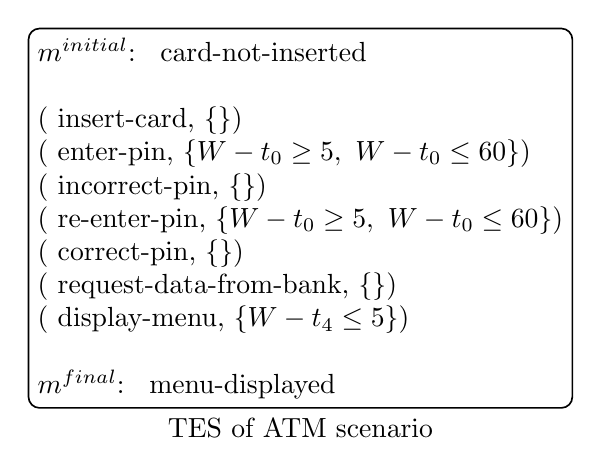
\begin{tikzpicture}[->,>=stealth']
			\tikzset{vertex/.style = {shape=rectangle,rounded corners, semithick, draw,align=left}}
			
			\node[vertex, label = below: TES of ATM scenario] (QUERY) 
			{ $m^{initial}$: { card-not-inserted} \\
				\\
				({ insert-card}, $\{\}$) \\
				({ enter-pin}, $\{W-t_0\geq 5,~W-t_0\leq 60\}$) \\
				({ incorrect-pin}, $\{\}$) \\
				({ re-enter-pin}, $\{W-t_0\geq 5,~W-t_0\leq 60\}$) \\
				({ correct-pin}, $\{\}$) \\
				({ request-data-from-bank}, $\{\}$) \\
				({ display-menu}, $\{W-t_4\leq 5\}$) \\
				\\
				$m^{final}$: { menu-displayed}
			};
			
			\end{tikzpicture}
			\end{adjustbox}
		\end{column}
	\end{columns}
	
\end{frame}

\begin{frame}{Dominance Assumption}
	\begin{itemize}
		\item Given two modes $m_i$ and $m_j$, $m_i$ is said to be the \emph{dominating mode} of $m_j$ iff all the paths to $m_j$ from the initial mode in the mode graph pass through $m_i$. We call this the \emph{Dominance} relation and denote it as \emph{$m_i$ DOM $m_j$}.
		\item Dominance assumption ensures that time variables are well defined.
	\end{itemize}
\end{frame}


\begin{frame}{Dominance Assumption Example}
	\begin{columns}
		\begin{column}{0.5\textwidth}
		\begin{figure}[!h]
	%	\begin{minipage}[b]{.3\textwidth}
			\begin{adjustbox}{max totalsize={.99\textwidth}{.65\textheight},center}
			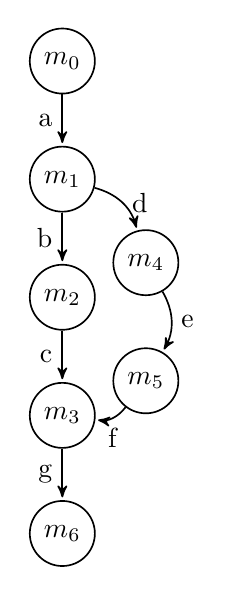
\begin{tikzpicture}[->,>=stealth',shorten >=1pt,auto,node distance=1.5cm,
			semithick]
			\tikzstyle{every state}=[draw,minimum size=1em]
			
			\node[state]       (S_0)                    {$m_0$};
			\node[state]         (S_1) [below of=S_0]     {$m_1$};
			\node[state]         (S_2) [below of=S_1]     {$m_2$};
			\node[state]         (S_3) [below of=S_2]     {$m_3$};
			\node[state]         (S_4) [below right of=S_1]   {$m_4$};
			\node[state]         (S_5) [below  of=S_4]    {$m_5$};
			\node[state]         (S_6) [below of=S_3]     {$m_6$};
				
			\path (S_0) edge              node[left]  {a}  (S_1)
			(S_1) edge              node[left]  {b}  (S_2)
			(S_2) edge              node[left]  {c}  (S_3)
			(S_1) edge [bend left]  node[right] {d}  (S_4)
			(S_4) edge [bend left]  node[right] {e}  (S_5)
			(S_5) edge [bend left]  node[below] {f}  (S_3)
			(S_3) edge              node[left]  {g}  (S_6)
			
			;
			\end{tikzpicture}
			\end{adjustbox}
		\end{figure}
		\end{column}
		\begin{column}{0.5\textwidth}
		\begin{figure}

			\begin{adjustbox}{max totalsize={.80\textwidth}{.80\textheight},center}
			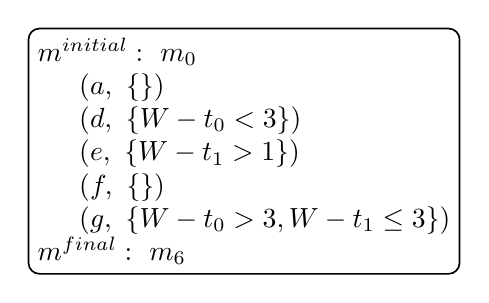
\begin{tikzpicture}[->,>=stealth']
			\tikzset{vertex/.style = {shape=rectangle,rounded corners, semithick, draw,align=left}}
			\node[vertex] (QUERY) 
			{$m^{initial}:~m_0$ \\
				
				\indent    ($a,~\{\}$) \\
				\indent    ($d,~\{W-t_0 < 3\}$) \\
				\indent    ($e,~ \{W-t_1 > 1\}$) \\
				\indent    ($f,~\{\}$) \\
				\indent   ($g,~\{W-t_0 > 3, W-t_1\leq 3\}$) \\
				
				$m^{final}:~m_6$};
			\end{tikzpicture}		
			\end{adjustbox}
	%		\caption{A mode graph and a scenario satisfying the dominance assumption}
	%		\label{fig:Dominance Assumption}
			\end{figure} 
		\end{column}
	\end{columns}
	\begin{itemize}
		\item $m_0$ and $m_1$ are dominating modes of $m_3$,
		\item Transition $g$ is dominated by all the modes that dominate $m_3$,
		\item $t_0$ and $t_1$, on transition $g$ refer to the time of leaving $m_0$ and $m_1$.
	\end{itemize}
\end{frame}

\begin{frame}{Constructing a Time Annotated Graph from Scenarios}
	Given a mode graph $\mathcal{M}$ and a set of Timed Event Sequences  $\Xi = \{\xi_1,\xi_2,..,\xi_k\}$ as inputs, we propose an algorithm for synthesizing a time annotated graph (TAG) G. Initially we start with an empty graph, $G_0$ and perform the following steps:
	\begin{enumerate}
		\item Build a partial graph $G_1$ using the first scenario $\xi_1$,
		\item The algorithm repeatedly takes a partially built graph $G_k$, and a scenario $\xi_{k+1} ~(1 < k < n)$ and then generates a new partial graph $G_{k+1}$.
	\end{enumerate}
	%\pause
	Decision on whether to create new states and transitions is resolved with the help of state labels (modes).
	A new state $s$ is created and labelled with a mode $m_j$ if there is an event $e$ from state $q$ such that $L(q) = m_i$ and $(m_i,e,m_j) \in T$.
\end{frame}

\begin{frame}{Properties of Constructed Time Annotated Graph}
The graph constructed by our algorithm has the following properties:
	\begin{enumerate}
		\item
		It is acyclic,%: as we do not introduce a transition from a state to it's previous states.
		%\pause
		\item
		It is connected,%, because the input set of TES is complete.
		%\pause
		\item\label{p3}
		By construction, two states have the same label only if one is a predecessor of the other, %We create a new state with the same label only to avoid introducing a transition from a state to it's predecessor.
		%\pause
		\item\label{p4} It is finite,
%		There must be at least one state with no outgoing transitions, because the graph is finite.
		%\pause
		\item
		It is deterministic,%: we only add a new transition only if it does not exist from state $s$.
		%\pause
		\item
		It is minimal, %because:
%		\begin{itemize}
%			\item
%			We do not add additional states if the state with mode information $m_i$ already exists. We only add in cases when the addition of a new transition creates a cycle.
%			\item
%			In case of multiple existing states, we choose the state that was created first.
%		\end{itemize}
		%\pause
		\item
		After construction, every scenario is a partial run of the constructed graph, and
		%\pause
		\item
		For every path in the constructed graph there is a corresponding path in the mode graph. %because our algorithm adds a new state or transition based on the mode and transition information in the mode graph.
	\end{enumerate}

\end{frame}


\begin{frame}{Constructing a Timed Automaton from Time Annotated Graph}
	After constructing the time annotated graph, we need to transform it to the target timed automaton. For that, the following steps should be performed in order:
	\begin{enumerate}	
		\item Determine the required number of clocks,
		\item Generate clock resets and clock constraints, and
		\item Add the clock resets and constraints to the appropriate transitions in the time annotated graph. %Replace the time annotations with the clock constraints
	\end{enumerate}
	\underline{Example}: If there is a time annotation $W-t_0 > 5$ on a transition, then the clock constraint $c_0 > 5$ is added to that transition and clock $c_0$ is reset on all transitions from the state labelled with mode $m_0$.
\end{frame}

\begin{frame}{Example of Synthesis Method}
	\begin{figure}
		\begin{adjustbox}{max totalsize={.99\textwidth}{.90\textheight},center}
		%	\begin{minipage}{.7\textwidth}
		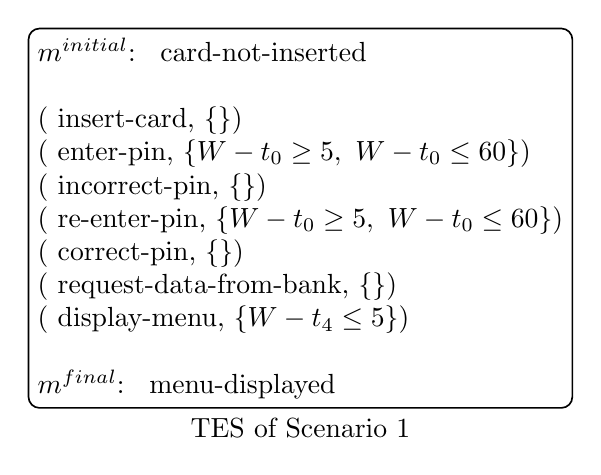
\begin{tikzpicture}[->,>=stealth']
		\tikzset{vertex/.style = {shape=rectangle,rounded corners, semithick, draw,align=left}}
		
		\node[vertex, label = below: TES of Scenario 1] (QUERY) 
		{ $m^{initial}$: { card-not-inserted} \\
			\\
			({ insert-card}, $\{\}$) \\
			({ enter-pin}, $\{W-t_0\geq 5,~W-t_0\leq 60\}$) \\
			({ incorrect-pin}, $\{\}$) \\
			({ re-enter-pin}, $\{W-t_0\geq 5,~W-t_0\leq 60\}$) \\
			({ correct-pin}, $\{\}$) \\
			({ request-data-from-bank}, $\{\}$) \\
			({ display-menu}, $\{W-t_4\leq 5\}$) \\
			\\
			$m^{final}$: { menu-displayed}
		};
		
		\end{tikzpicture}
		%\end{minipage}
		\hspace{0.5cm}
		%	\begin{minipage}{.7\textwidth}
		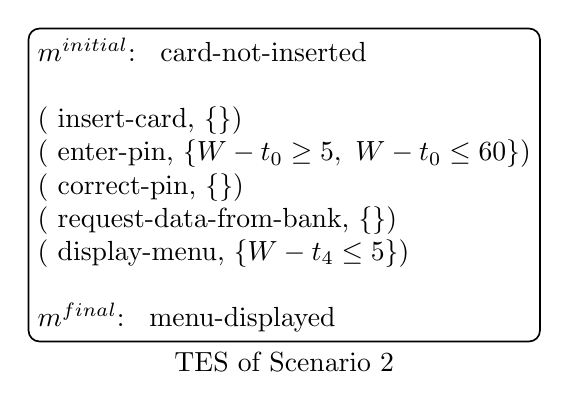
\begin{tikzpicture}[->,>=stealth']
		\tikzset{vertex/.style = {shape=rectangle,rounded corners, semithick, draw,align=left}}
		\node[vertex, label = below: TES of Scenario 2] (QUERY) 
		{ $m^{initial}$: { card-not-inserted} \\
			\\
			({ insert-card}, $\{\}$) \\
			({ enter-pin}, $\{W-t_0\geq 5,~W-t_0\leq 60\}$) \\
			({ correct-pin}, $\{\}$) \\
			({ request-data-from-bank}, $\{\}$) \\
			({ display-menu}, $\{W-t_4\leq 5\}$) \\
			\\
			$m^{final}$: { menu-displayed}
		};
		
		\end{tikzpicture}
		%	\end{minipage}
		\end{adjustbox}
		\caption{Timed Event Sequences of the ATM}
		\label{fig:TES of ATM}
	\end{figure}
\end{frame}

\begin{frame}{Example (Cont.)}

	 \begin{figure}[htp]
		 \centering
		 \includegraphics[width=0.9\columnwidth,height=0.8\textheight]{"ModeGraph"}
		 \caption{Mode Graph for ATM}
		 \label{fig:Mode Graph for ATM}
	 \end{figure}
\end{frame}

\begin{frame}{Example (Synthesized Graph and Timed Automaton)}
	\begin{columns}[T]
		\begin{column}{0.5\textwidth}
			\begin{figure}
				\begin{adjustbox}{max totalsize={.99\textwidth}{.85\textheight},center}
					\begin{tikzpicture}[->,>=stealth',shorten >=1pt,auto,node distance=2.5cm,
					semithick,font=\Large]
					\tikzstyle{every state}=[shape=rectangle,draw,minimum size=1cm]
					
					\node[state]       (S_0)                {$S_0$[$m_0$]};
					\node[state]         (S_1) [below of=S_0] {$S_1$[$m_1$]};
					\node[state]         (S_2) [below of=S_1] {$S_2$[$m_2$]};
					\node[state]         (S_3) [below of=S_2] {$S_3$[$m_3$]};
					\node[state]         (S_4) [below of=S_3] {$S_4$[$m_2$]};
					\node[state]         (S_5) [below of=S_4] {$S_5$[$m_4$]};
					\node[state]         (S_6) [below of=S_5] {$S_6$[$m_5$]};
					\node[state]         (S_7) [below of=S_6] {$S_7$[$m_6$]};
					
					
					\path (S_0) edge              node[left] {insert-card}                (S_1)
					(S_1) edge              node[left] {enter-pin [$W − t_0 \ge 5, W − t_0 \le 60$]}  (S_2)
					(S_2) edge        node[left] {incorrect-pin}              (S_3)
					(S_3) edge              node[left] {enter-pin [$W − t_0 \ge 5, W − t_0 \le 60$]}  (S_4)
					(S_4) edge              node[left] {correct-pin} (S_5)
					(S_5) edge        node[left] {request-data-from-bank} (S_6)
					(S_6) edge        node[left] {display-menu [$W − t_4 \le 5$]} (S_7)
					(S_2) edge [bend left]  node[right] {correct-pin} (S_5)
					;
					\end{tikzpicture}
			
				\end{adjustbox}
%				\caption{Time annotated graph synthesized from two TES in Figure \ref{fig:TES of ATM}}
%				\label{fig:Time annotated graph generated by combining scenario 1 and scenario 2}
			\end{figure}			
		\end{column}
	
		\begin{column}{0.5\textwidth}
			\begin{figure}[!htb]
				\begin{adjustbox}{max totalsize={.99\textwidth}{.9\textheight},center}
					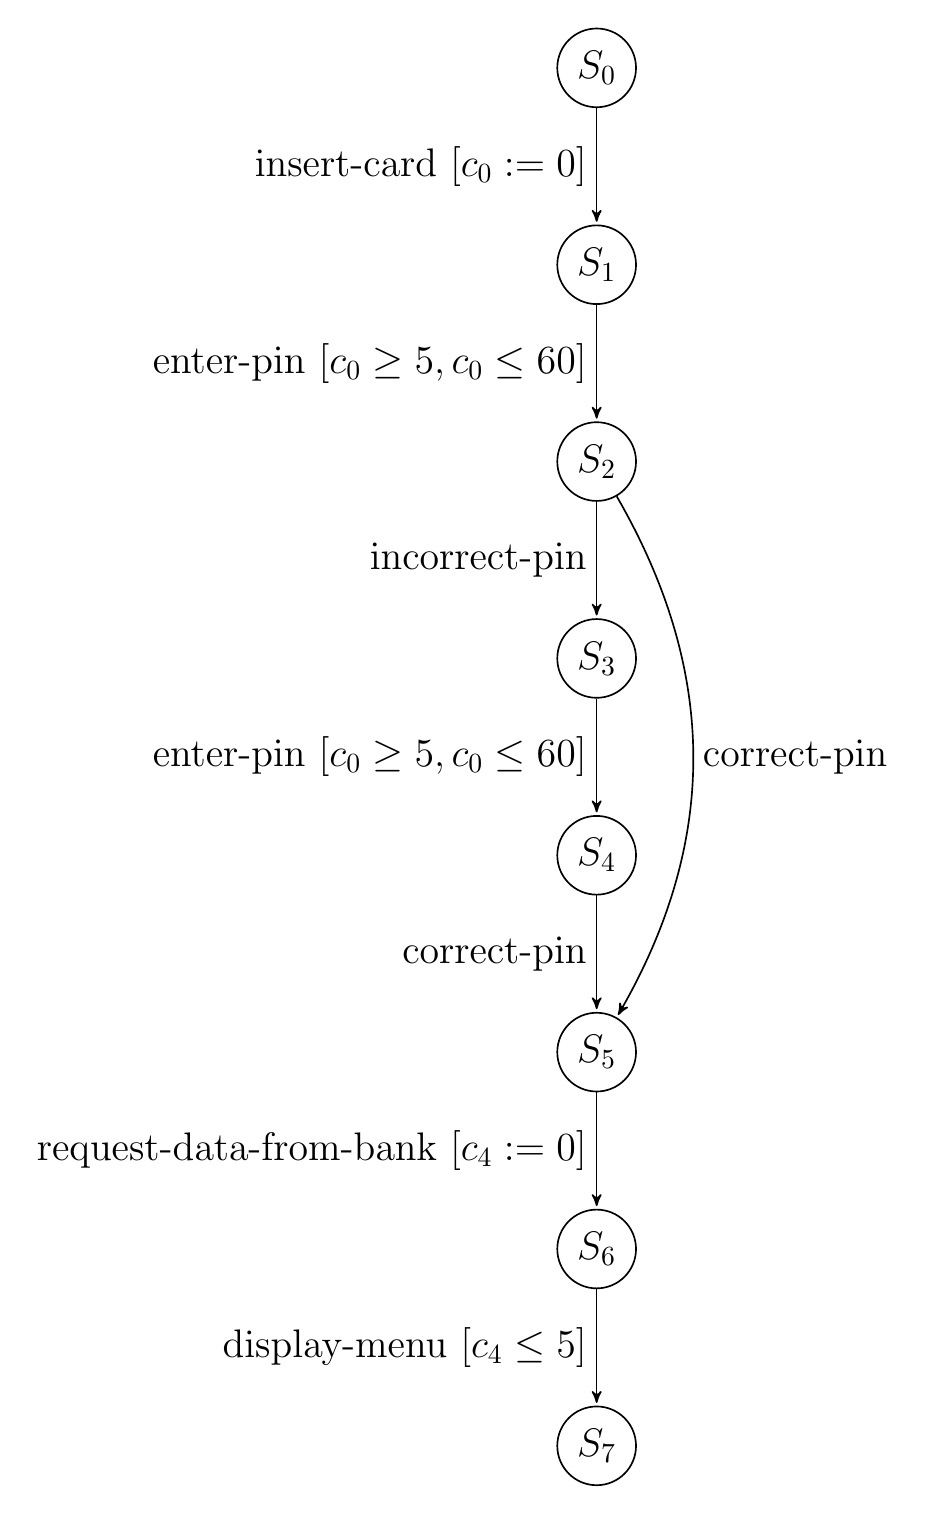
\begin{tikzpicture}[->,>=stealth',shorten >=1pt,auto,node distance=2.5cm,
					semithick,font=\Large]
					\tikzstyle{every state}=[draw,minimum size = 1cm]
					
					\node[state]       (S_0)                {$S_0$};
					\node[state]         (S_1) [below of=S_0] {$S_1$};
					\node[state]         (S_2) [below of=S_1] {$S_2$};
					\node[state]         (S_3) [below of=S_2] {$S_3$};
					\node[state]         (S_4) [below of=S_3] {$S_4$};
					\node[state]         (S_5) [below of=S_4] {$S_5$};
					\node[state]         (S_6) [below of=S_5] {$S_6$};
					\node[state]         (S_7) [below of=S_6] {$S_7$};
					
					
					\path (S_0) edge              node[left] {insert-card [$c_0 :=0$]}                (S_1)
					(S_1) edge              node[left] {enter-pin [$c_0 \ge 5, c_0 \le 60$]}  (S_2)
					(S_2) edge        node[left] {incorrect-pin}              (S_3)
					(S_3) edge              node[left] {enter-pin [$c_0 \ge 5, c_0 \le 60$]}  (S_4)
					(S_4) edge              node[left] {correct-pin} (S_5)
					(S_5) edge        node[left] {request-data-from-bank [$c_4 :=0$]} (S_6)
					(S_6) edge        node[left] {display-menu [$c_4 \le 5$]} (S_7)
					(S_2) edge [bend left]  node[right] {correct-pin} (S_5)
					;
					\end{tikzpicture}
				\end{adjustbox}
%				\caption{Timed automaton constructed from time annotated graph in Figure \ref{fig:Time annotated graph generated by combining scenario 1 and scenario 2}}
%				\label{fig:Timed Automaton generated by combining scenario 1 and scenario 2}
			\end{figure}	
			
		\end{column}
	\end{columns}

\end{frame}

\subsection{Optimal Clock Allocation of Timed Automata}

\begin{frame}{Class of Timed Automata}
The timed automaton constructed as a result of our synthesis method belongs to the class of timed automata that satisfies these properties:
	\begin{enumerate}
		\item{The automaton is connected and has a unique initial state $s_0$,}%Every state is reachable from $s_0$},
		%\pause
		\item{A clock constraint on a transition `$r$' can only refer to the times of transitions from states that dominate the transition `$r$', we call this the \textit{dominance assumption}},
		%\pause
		\item{A clock $t_j$ can only be reset on a transition leaving a state $s$, where label is $j$, that is $L(s)=j$.}
		%\pause
	\end{enumerate}
\end{frame}

\begin{frame}{Optimal Clock Allocation of Timed Automata}
%	Given a timed automaton $\cal A$ that belongs to the aforementioned class of timed automata, to transform it to an equivalent timed automaton $\cal A'$ with optimal allocation of clocks, we need to perform the following steps in order:
	To optimally allocate clocks in a timed automaton $\cal A$ that belongs to our class of timed automata, we need to perform the following steps in order:
	\begin{enumerate}
		\item{Determine the liveness ranges of clocks in the timed automaton $\cal A$,}
		\item{Determine the minimum number of clocks required,}
		\item{Replace the original clocks in $\cal A$ with a set of new clocks,} %such that $|P|\le|V|$,}
		%\item{Replace the original clocks in $A ~(V=\left\{t_0,t_1,...,t_n \right\}$) with a set of new clocks $P=\left \{c_0,c_1,..,c_m \right\}$ such that $|P|\le|V|$}
		\item{Rewrite the clock constraints and clock resets in $\cal A$ in terms of new clock variables.}
	\end{enumerate}
%	As the problem of deciding if there exists another timed automaton accepting the same language as $\cal A$ is \emph{undecidable} in general, we do not take into account the satisfiability of clock constraints.
%The complexity of our optimal clock allocation algorithm is quadratic in the size of the original graph.

\end{frame}

\begin{frame}{Liveness Range Analysis}
Liveness Ranges of all the clocks in a timed automaton helps us determine if a particular clock is needed on these transitions.
\begin{itemize}
	\item Let $\cal A$ $= (E, Q, \{q^0\}, Q_f, V, R, L)$ be the timed automaton and $r = (s, s', e, \lambda_r, \phi_r) \in R$ be a transition.
	\item Let $N = \{j~|~t_j\sim a \in \phi \vee t_j \in \lambda$, where $(s, s', e, \lambda_r, \phi_r) \in R\}$, be a set of \emph{clock numbers} used to denote subscripts of the clocks on all the transitions in $R$.
\end{itemize}
\end{frame}

\begin{frame}{Liveness Range Analysis}
	The following are a set of functions used to calculate the liveness ranges:
	\begin{itemize}
		\item
		$\mathit{\textbf{clock\_ref}}$: $\mathit{clock\_ref(r)}$ is the set of clocks which are referred to in the clock constraints on $r$.
		%\pause
		\item
		$\textbf{born}$: $\Born(r)$ identifies a clock that is reset on $r$  whose value can be used on some transition	reachable from $r$.
		%\pause
		\item 
		$\textbf{active}$: $\Active(r)$ identifies clocks that are ``alive'' on $r$ (i.e., their  values may be subsequently used). Notice that $\Born(r)\subseteq \Active(r)$.
		%\pause
		\item
		$\textbf{needed}$: Maps transition $r$ to $\Active(r)\cup \mathit{clock\_ref(r)}$.
		
	\end{itemize}

\end{frame}

\begin{frame}{Liveness Analysis Algorithm}
\begin{adjustbox}{max totalsize={.99\textwidth}{.9\textheight},center}
\IncMargin{1em}
\begin{algorithm*}[H]
	\SetKwData{Left}{left}\SetKwData{This}{this}\SetKwData{Up}{up}
	\SetKwFunction{Union}{Union}\SetKwFunction{FindCompress}{FindCompress}
	\SetKwInOut{Input}{Input}\SetKwInOut{Output}{Output}
	\Input{A timed automaton ${\cal A} = \langle E, Q, \{q^0\}, Q_f, V, R, L \rangle$.}
	\Output{An extended timed automaton ${\cal A}_e = \langle E, Q, \{q^0\}, Q_f, V, R_e, L \rangle$, where $R_e$ is the set of extended transitions.}
	\BlankLine
	$R_e$ := $\emptyset$\;
	\ForEach{transition $r=(s, q, e, \phi) \in R$ in $\cal A$}
	{
		$\Var{born}(r)$ := $\Var{active}(r)$ := $\emptyset$\;
	}
	\Repeat{there were no changes}
	{
		\ForEach{transition $r=(s, q, e, \lambda, \phi) \in R$ in $\cal A$}
		{
			\ForEach{$r_o\in \Var{out(q)}$}
			{
				$\Var{active(r)}$ := $\Var{active}(r)\cup
				((\Var{active}(r_o) \cup
				\Var{clock\_ref}(r_o)) \setminus
				\Var{born}(r_o)) $\;
			}
			\If{$L(s) = j$ and $j\in \Var{active}(r)$}
			{
				$\Var{born}(r)$ := $\{j\}$\;
			}
			$R_e$ := $R_e \cup
			\{(r, \Var{born}(r), \Var{active}(r))\}$\;
		}
	}
	\caption{Building the liveness ranges for clocks}\label{clock-live}
\end{algorithm*}\DecMargin{1em}
\end{adjustbox}
\end{frame}

\begin{frame}{Liveness Range Analysis Example}
 \begin{columns}
	\begin{column}{0.4\textwidth}
		\begin{figure}
			\begin{adjustbox}{max totalsize={.99\textwidth}{.8\textheight}}
			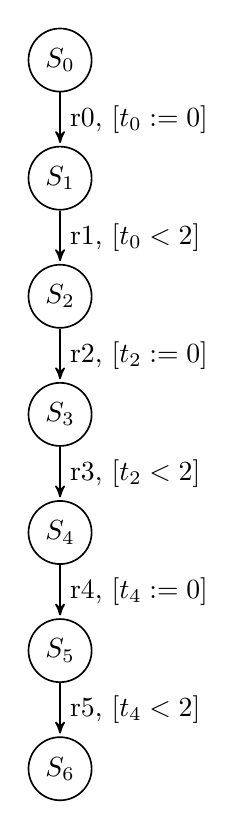
\begin{tikzpicture}[->,>=stealth',shorten >=1pt,auto,node distance=1.5cm,
			semithick]
			\tikzstyle{every state}=[draw,minimum size=1em]
			
			\node[state]         (S_0)                    {$S_0$};
			\node[state]         (S_1) [below of=S_0]     {$S_1$};
			\node[state]         (S_2) [below of=S_1]     {$S_2$};
			\node[state]         (S_3) [below of=S_2]     {$S_3$};
			\node[state]         (S_4) [below of=S_3]     {$S_4$};
			\node[state]         (S_5) [below of=S_4]     {$S_5$};
			\node[state]         (S_6) [below of=S_5]     {$S_6$};	
			
			\path (S_0) edge              node[right]  {r0, [$t_0:=0$]}  (S_1)
			(S_1) edge              node[right]  {r1, [$t_0<2$]}   (S_2)
			(S_2) edge              node[right]  {r2, [$t_2:=0$]}  (S_3)
			(S_3) edge              node[right] {r3, [$t_2<2$]}   (S_4)
			(S_4) edge              node[right] {r4, [$t_4:=0$]}  (S_5)
			(S_5) edge              node[right] {r5, [$t_4<2$]}   (S_6)
			
			;
			\end{tikzpicture}
			\end{adjustbox}
			\caption{A simple timed automaton}
			\label{fig:Simple Timed Automaton}
		\end{figure}
	\end{column}
			\begin{column}{0.5\textwidth}
			\begin{table}
				\centering
				\caption{$born$ and $active$ functions}
				\label{tab:table1}
				\begin{tabular}{ccc}
					\toprule
					{ \textbf{Transition}} & { \textbf{Born}} & { \textbf{Active}} \\ \midrule
					{ $r_0$}               & { \{0\}}         & { \{0\}}           \\
					{ $r_1$}               & { $\phi$}        & { $\phi$}          \\
					{ $r_2$}               & { \{2\}}         & { \{2\}}           \\
					{ $r_3$}               & { $\phi$}        & { $\phi$}          \\
					{ $r_4$}               & { \{4\}}         & { \{4\}}           \\
					{ $r_5$}               & { $\phi$}        & { $\phi$} \\
					\bottomrule
				\end{tabular}
			\end{table}
		\end{column}
		\begin{column}{0.1\textwidth}
		\end{column}
	\end{columns}
\end{frame}

\begin{frame}{Clock Allocation}
	Our liveness analysis algorithm calculates the liveness ranges of clocks and generates extended transitions of the form $(r,born(r),active(r))$. \\
	\vspace{0.5cm}
	Our method to optimally allocate the clocks revolves around the idea that: 
	\begin{itemize}
		\item A clock can be reused if the active range of the clock has ended,
		\item The clock cannot be reused on a transition if the transition belongs to active range of that clock.
	\end{itemize}

\end{frame}

\begin{frame}{Clock Allocation}
%	\begin{definition}	
	\textbf{Definition:} Given a timed automaton $\cal A$ with the set $R$ of (extended) transitions and the set $N$ of clock numbers, a \emph{clock allocation} for $\cal A$ is a relation $\Var{alloc}\subset R\times P_0\times N$ such that $(r, c, j)\in \Var{alloc} \Rightarrow j\in \Var{active(r)}$. Where, $P_0$ is the pool of new clock variables.
%	\end{definition}
	%\pause
	\begin{columns}
		\begin{column}{0.5\textwidth}
			\begin{figure}[!h]
				\begin{adjustbox}{max totalsize={.99\textwidth}{.65\textheight},center}
					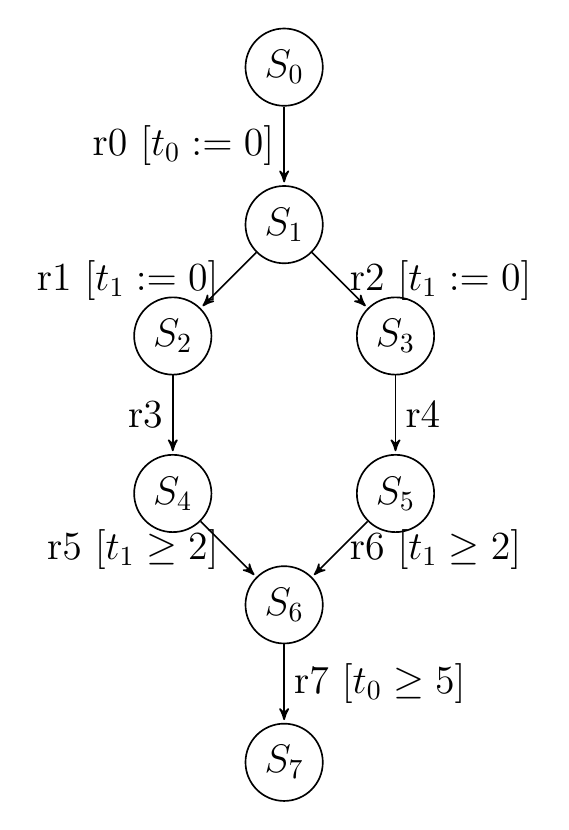
\begin{tikzpicture}[->,>=stealth',shorten >=1pt,auto,node distance=2cm,
					semithick,font=\Large]
					\tikzstyle{every state}=[draw,minimum size=1em]
					
					\node[state]         (S_0)                    {$S_0$};
					\node[state]         (S_1) [below of=S_0]     {$S_1$};
					\node[state]         (S_2) [below left of=S_1]     {$S_2$};
					\node[state]         (S_3) [below right of=S_1]     {$S_3$};
					\node[state]         (S_4) [below of=S_2]   {$S_4$};
					\node[state]         (S_5) [below  of=S_3]    {$S_5$};
					\node[state]         (S_6) [below left of=S_5]     {$S_6$};
					\node[state]         (S_7) [below of=S_6]     {$S_7$};
					
					
					
					\path (S_0) edge              node[left]  {r0 [$t_0 := 0$]}  (S_1)
					(S_1) edge              node[left]  {r1 [$t_1 := 0$]}  (S_2)
					(S_1) edge              node[right] {r2 [$t_1 := 0$]}  (S_3)
					(S_2) edge              node[left]  {r3 }  (S_4)
					(S_3) edge              node[right] {r4 }  (S_5)
					(S_4) edge              node[left]  {r5 [$t_1\ge2$]}  (S_6)
					(S_5) edge              node[right] {r6 [$t_1\ge2$]}  (S_6)
					(S_6) edge              node[right] {r7 [$t_0\ge5$]}  (S_7)
					
					
					;
					\end{tikzpicture}
				\end{adjustbox}
%				\caption{A timed automaton satisfying the dominance assumption}
%				\label{fig:SimpleTimedAutomaton2}
			\end{figure}
		\end{column}
		\begin{column}{0.5\textwidth}
			$\Var{alloc}~$=$\{(r_0,c_0,0), (r_1,c_0,0), (r_2,c_0,0), $\\ $(r_3,c_0,0),(r_4,c_0,0), (r_5,c_0,0), (r_6,c_0,0), $\\$(r_1,c_1,1),(r_2,c_1,1), (r_3,c_1,1), (r_4,c_1,1)\} $
		\end{column}
		
	\end{columns}

\end{frame}

\begin{frame}{Problematic States}

	\begin{figure}
		\begin{adjustbox}{max totalsize={.99\textwidth}{.5\textheight},center}
		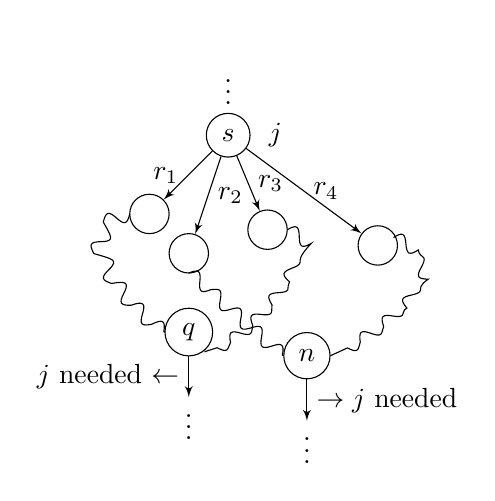
\begin{tikzpicture}		
		\tikzset{vertex/.style = {shape=circle,draw,minimum size=0.5cm}}
		\tikzset{vertex2/.style = {shape=circle,draw=none,minimum size=0.5cm}}
		\tikzset{edge/.style = {->,> = latex'}}
		% vertices
		\node[vertex] (a) at  (0,0) {$s$};
		\node[vertex] (b) at  (-1,-1) {};
		\node[vertex] (c) at  (-0.5,-1.5) {};
		\node[vertex] (d) at  (0.5,-1.2) {};
		\node[vertex] (e) at  (1.9,-1.4) {};
		
		\node[vertex] (f) at  (-0.5,-2.5) {$q$};
		\node[vertex] (g) at  (1,-2.8) {$n$};
		
		\node[vertex2] (bm) at  (0.6,0) {$j$};
		%\node[vertex2] (label) at  (0,-4.7) {(b)};
		
		\node [shape=circle,minimum size=0.5em] (a1) at (0,1.2) {};
		
		\node [shape=circle,minimum size=0.5em] (c1) at (-0.5,-3.5) {};
		\node [shape=circle,minimum size=0.5em] (c2) at (-0.5,-3.7) {};
		
		\node [shape=circle,minimum size=0.5em] (d1) at (1,-3.8) {};
		\node [shape=circle,minimum size=0.5em] (d2) at (1,-4) {};
		
		\draw[edge] (f) to node[left]{$j$ needed $\leftarrow $} (c1) ;
		\draw[edge] (g) to node[right]{$\rightarrow j$ needed} (d1) ;
		
		\path (c1) to node {\vdots} (c2);
		\path (d1) to node {\vdots} (d2);
		
		%edges
		\draw[edge] (a) to node[left]{$r_1$} (b) ;
		\draw[edge] (a) to node[right]{$r_2$} (c) ;
		\draw[edge] (a) to node[right]{$r_3$} (d) ;
		\draw[edge] (a) to node[right]{$r_4$} (e) ;
		
		\path (a1) to node {\vdots} (a);
		
		\draw [decorate, decoration={coil,aspect=0}]
		{ (-1.25,-1) .. controls (-1.9,-1.2) and (-1.5,-2) .. (-0.8,-2.5) };
		
		\draw [decorate, decoration={coil,aspect=0}]
		{ (0.75,-1.2) .. controls (1.1,-1.4) and (0.5,-2.5) .. (-0.3,-2.75) };
		
		\draw [decorate, decoration={coil,aspect=0}]
		{ (-0.5,-1.75) .. controls (-0.3,-1.9) and (0,-2.2) .. (0.7,-2.8) };
		
		\draw [decorate, decoration={coil,aspect=0}]
		{ (2.1,-1.3) .. controls (2.9,-1.7) and (2,-2.5) .. (1.3,-2.8) };
		\end{tikzpicture}
		\end{adjustbox}
		\caption{A timed automaton with problematic states}
%		\label{twofamilies}		
	\end{figure}
%	Consider example shown in Figure \ref{twofamilies}:
	\begin{itemize}
		\item Clock $t_j$ is born on all outgoing transitions of state $s$.
		\item $r_1$, $r_3$ meet at state $q$ and $r_2$, $r_4$ meet at state $n$.
	\end{itemize}
	%\pause
	States $q$ and $n$ are the \emph{problematic} states. So, $r_1,r_3$ should be assigned the same clock and $r_2,r_4$ should be assigned the same clock.
\end{frame}

\begin{frame}{Handling the Problematic States}
	To handle the problematic states, we partition the transitions into mothers and others.
		\begin{itemize}
			\item $mothers$: $\{r \in \Var{out(s)}~ |~ j \in \Var{born(r)}\}$
			\item $others$: $\{r \in \Var{out(s)}~ |~ \Var{born(r)} = \emptyset\}$
		\end{itemize}
	%\pause
	We use the following functions:
		\begin{itemize}
			\item
			$\Var{reachable}: Q\rightarrow 2^{Q}$ maps state $q$ to the set of states that are reachable from $q$ by some non-empty path.
			\item
			$\Var{reachable\_from}: Q\rightarrow 2^{Q}$ maps state $q$ to the set of states from which it can be reached by some non-empty path.
		\end{itemize}
\end{frame}

%\begin{frame}{Handling the Problematic States (Contd..)}
%
%	\Var{PP} := $\emptyset$; $~~~~~~\slash\slash$ potentially problematic states
%	
%	\ForEach{$r\in \Var{mothers}$}
%	{
%		\ForEach{$s\in \Var{reachable(target(r))}$}
%		{
%			\If{$L(q)\in \Var{active(r')}$, where $r'$ is an arbitrary transition of $\Var{in(s)}$}
%			{
%				\Var{PP} := $\Var{PP}\cup \{s\}$\;
%			}
%		}
%	}
%
%	%\pause
%	Those states in \Var{PP} that can be reached from more than one mother are the problematic states.
%
%\end{frame}

\begin{frame}{Clock Allocation Algorithm}
	\begin{procedure}[H]
		\SetKwData{Left}{left}\SetKwData{This}{this}\SetKwData{Up}{up}
		\SetKwFunction{Union}{Union}\SetKwFunction{FindCompress}{FindCompress}
		\SetKwInOut{Input}{Input}\SetKwInOut{Output}{Output}
		\Input{An extended timed automaton
			${\cal A}_e = \langle E, Q, \{q^0\}, Q_f, V, R_e, L \rangle$\\
			and the initial pool of available clocks, $P_0$.}
		\Output{An extended timed automaton
			${\cal A}'_e = \langle E, Q_e, \{q^0\}, Q_f, V, R_e, L \rangle$,\\
			where $Q_e = Q\times 2^{P_0}\times 2^{P_0\times N}$.}
		
		\ForEach{state $s\in Q$}
		{
			Set the status of $s$ to $\Unseen{}$\;
		}
		$\Var{annotate(q^0, P_0, \emptyset)}$\;
		
		$\Var{visit(q^0)}$\;
		\caption{compute-allocation(timed automaton ${\cal A}_e$, set of clocks $P_0$)}
		\label{clock-main}
	\end{procedure}
	
\end{frame}

\begin{frame}{Clock Allocation Algorithm (Contd..)}
	\begin{procedure}[H]
		%$\slash\slash$ Annotating states with pool of available clocks and \\
		%$\slash\slash$ clock assignments
		
		$\slash\slash$ Invoked only when status of $q$ is \Unseen{}.
		
		$\Var{pool(q)}$ := $p$\;
		
		$\Var{assignments(q)}$ := $\cal a$\;
		
		Set the status of $q$ to $\Seen{}$\;
		\caption{annotate(state $q$, set of clocks $p$, set of assignments $\cal a$)}
		\label{proc:clock-annotate}
	\end{procedure}

	\begin{procedure}[H]
		
		$\slash\slash$ Invoked only when the status of $q$ is \Seen{} or \Visited{}.
		
		\If{status of $q$ is not $\Visited{}$}
		{
			Set the status of $q$ to $\Visited{}$\;
			
			\emph{annotate-immediate-successors-of}($q$)\;
			
			\ForEach{$r\in \Var{out(q)}$}
			{
				$\Var{visit(target(r))}$\;
			}
		}
		\caption{visit(state $q$)}
		\label{proc:visit}
	\end{procedure}
\end{frame}
	
\begin{frame}{Clock Allocation Algorithm (Contd..)}
	\begin{procedure*}[H]
		
		Partition $\Var{out(q)}$ into $\Var{mothers}$ and $\Var{others}$\;
		
		\ForEach{$r\in \Var{others}$}
		{
			\If{status of $\Var{target(r)}$ is $\Unseen{}$}
			{
				propagate($q, r, \emptyset$)\;
			}
			$\slash\slash$ Otherwise $\Var{target(r)}$ is already properly annotated                     %:see Theorem~\ref{alloc}.
		}
		\If{$\Var{mothers}\neq \emptyset$}
		{
			$\Var{Groups}$ := 
			\PartitionIntoASetOfGroups($q, \Var{mothers}$)\;
			
			\ForEach{$\Var{group}\in \Var{Groups}$}
			{
				$c$ := \Var{find}-\Var{clock}($q, \Var{group}$)\;
				
				\ForEach{$r\in \Var{group}$}
				{
					$\slash\slash$ The target of $r$ is \Unseen{} (by the dominance assumption).
					
					$\Var{propagate(q, r, \{c\})}$\;
				}
			}
		}
		\caption{annotate-immediate-successors-of(state $q$)}
		\label{proc:clock-annotate-successors}
	\end{procedure*}
\end{frame}

\begin{frame}{Clock Allocation Algorithm (Contd..)}
	\begin{procedure*}[H]
		
		$\slash\slash$ $q$ is the source of $r$. Propagate $\Var{pool(q)}$ and
		$\Var{assignments(q)}$ to $\Var{target(r)}$, taking into account that some
		clock ranges \\
		$\slash\slash$ may end on $r$. If $sc$ is not empty, it must be a
		singleton: in that case assign its member to clock number $L(q)$.
		
		$\slash\slash$ Invoked only when the target of $r$ is \Unseen{}.
		
		%$\slash\slash$ The set of assignments for ranges dying in $r$:
		
		\Var{freed\_assignments} := $\{(d, j)~|~(d, j)\in \Var{assignments(q)} \wedge j\notin \Var{active(r)}\}$\;
		
		%$\slash\slash$ The set of clocks whose associated ranges dying in $r$:
		
		\Var{freed\_clocks} := $\{d~|~(d, j)\in \Var{freed\_assignments}\}$\;
		
		\Var{tmp\_pool} := $\Var{pool(q)}\cup \Var{freed\_clocks}$\;
		
		\Var{tmp\_assignments} := $\Var{assignments(q)}\setminus \Var{freed\_assignments}$\;
		
		\If{$\Var{sc} \neq \emptyset$}
		{
			\Var{tmp\_pool} := $\Var{tmp\_pool} \setminus \Var{sc}$\;
			\Var{tmp\_assignments} := $\Var{tmp\_assignments} \cup \{(c, L(q))\}$, where $c \in \Var{sc}$\;
		}
		
		$\Var{annotate( target(r), tmp\_pool, tmp\_assignments)}$\;
		
		\caption{propagate(state $q$, transition $r$, set of clocks $sc$)}
		\label{proc:clock-propagate}
	\end{procedure*}
\end{frame}

\begin{frame}{Clock Allocation Algorithm (Contd..)}
	\begin{adjustbox}{max totalsize={.99\textwidth}{.95\textheight}}
	\begin{procedure*}[H]
		
		$\mathit{mother\_targets}$ := $\{\Var{target(r)}~|~r\in \Var{mothers}\}$\;
		
		$\slash\slash$ Initially, each mother is in its own group.
		
		\Var{Groups} := $\emptyset$\;
		
		\ForEach{$r\in \Var{mothers}$}
		{
			\Var{Groups} := $\Var{Groups} \cup \{r\}$\;
		}
		\Var{PP} := $\emptyset$; $~~~~~~\slash\slash$ potentially problematic states
		
		\ForEach{$r\in \Var{mothers}$}
		{
			\ForEach{$s\in \Var{reachable(target(r))}$}
			{
				\If{$L(q)\in \Var{active(r')}$, where $r'$ is an arbitrary transition of $\Var{in(s)}$}
				{
					\Var{PP} := $\Var{PP}\cup \{s\}$\;
				}
			}
		}
		$\slash\slash$ Those states in \Var{PP} that can be reached from more than one mother are the problematic states.
		
		\ForEach{$s\in \Var{PP}$}
		{
			\Var{targets} := $\mathit{reachable\_from(s)} \cap \mathit{mother\_targets}$\;
			
			Merge those members of \Var{Groups} that contain transitions whose target is in \Var{targets};
		}
		return \Var{Groups}\;
		\caption{partition-into-a-set-of-groups(state $q$, set of transitions \Var{mothers})}
		\label{clock-partition}
	\end{procedure*}
	\end{adjustbox}
\end{frame}

\begin{frame}{Clock Allocation Algorithm (Contd..)}
	\begin{procedure*}[H]
		$\slash\slash$ Find a clock for $L(q)$ on transitions in $group$.
		
		$\mathit{live\_on\_entry}$ := $\{j~|~(c, j)\in \Var{assignments(q)}\}$\;
		
		$\mathit{dying\_all}$ := $\bigcap_{r\in \Var{group}} (\mathit{live\_on\_entry} \setminus \Var{active(r)})$\;
		
		$\slash\slash$ The set of clocks whose liveness ranges end in all the
		transitions in $\Var{group}$:
		
		$\mathit{released\_all}$ :=
		$\{c~|~(c, j)\in \Var{assignments(q)}\wedge j\in \mathit{dying\_all}\}$\;
		
		$\Var{available}$ := $\mathit{released\_all} \cup \Var{pool(q)}$\;
		
		Return the clock variable with the smallest number in \Var{available}\;
		\caption{find-clock(state $q$, set of transitions \Var{group})}
		\label{proc:clock-find}
	\end{procedure*}
\end{frame}

\begin{frame}{Example: Optimal Clock Allocation}
	\begin{columns}[T]
		\begin{column}{0.5\textwidth}
			\begin{figure}
				\begin{adjustbox}{max totalsize={.90\textwidth}{.75\textheight},center}
					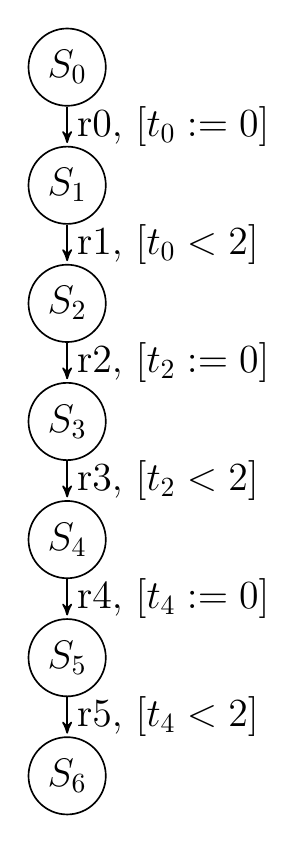
\begin{tikzpicture}[->,>=stealth',shorten >=1pt,auto,node distance=1.5cm,
					semithick,font=\Large]
					\tikzstyle{every state}=[draw,minimum size=1em]
					
					\node[state]         (S_0)                    {$S_0$};
					\node[state]         (S_1) [below of=S_0]     {$S_1$};
					\node[state]         (S_2) [below of=S_1]     {$S_2$};
					\node[state]         (S_3) [below of=S_2]     {$S_3$};
					\node[state]         (S_4) [below of=S_3]     {$S_4$};
					\node[state]         (S_5) [below of=S_4]     {$S_5$};
					\node[state]         (S_6) [below of=S_5]     {$S_6$};
					
					
					
					\path (S_0) edge              node[right]  {r0, [$t_0:=0$]}  (S_1)
					(S_1) edge              node[right]  {r1, [$t_0<2$]}   (S_2)
					(S_2) edge              node[right]  {r2, [$t_2:=0$]}  (S_3)
					(S_3) edge              node[right] {r3, [$t_2<2$]}   (S_4)
					(S_4) edge              node[right] {r4, [$t_4:=0$]}  (S_5)
					(S_5) edge              node[right] {r5, [$t_4<2$]}   (S_6)
					
					;
					\end{tikzpicture}
				\end{adjustbox}
			\caption{A simple timed automaton}
%			\label{fig:Simple Timed Automaton}				
			\end{figure}
		\end{column}
		\begin{column}{0.5\textwidth}
			\begin{figure}
				\begin{adjustbox}{max totalsize={.99\textwidth}{.75\textheight},center}
					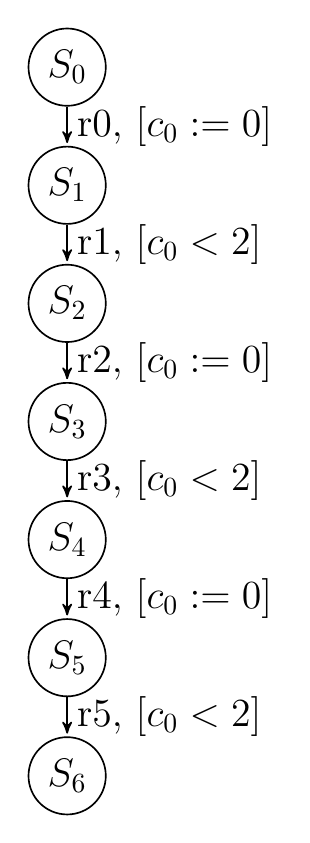
\begin{tikzpicture}[->,>=stealth',shorten >=1pt,auto,node distance=1.5cm,
					semithick,font=\Large]
					\tikzstyle{every state}=[draw,minimum size=1em]
					
					\node[state]         (S_0)                    {$S_0$};
					\node[state]         (S_1) [below of=S_0]     {$S_1$};
					\node[state]         (S_2) [below of=S_1]     {$S_2$};
					\node[state]         (S_3) [below of=S_2]     {$S_3$};
					\node[state]         (S_4) [below of=S_3]     {$S_4$};
					\node[state]         (S_5) [below of=S_4]     {$S_5$};
					\node[state]         (S_6) [below of=S_5]     {$S_6$};
					
					
					
					\path (S_0) edge              node[right]  {r0, [$c_0:=0$]}  (S_1)
					(S_1) edge              node[right]  {r1, [$c_0<2$]}   (S_2)
					(S_2) edge              node[right]  {r2, [$c_0:=0$]}  (S_3)
					(S_3) edge              node[right] {r3, [$c_0<2$]}   (S_4)
					(S_4) edge              node[right] {r4, [$c_0:=0$]}  (S_5)
					(S_5) edge              node[right] {r5, [$c_0<2$]}   (S_6)
					
					;
					\end{tikzpicture}
				\end{adjustbox}
			\caption{A simple optimally allocated timed automaton}
%			\label{fig:Simple Optimal Timed Automaton}
			\end{figure}
		\end{column}
	\end{columns}
\end{frame}

\section{Case Studies}

\begin{frame}{Automated Teller Machine (ATM)}
	We use an invariant of an ATM:
	\begin{enumerate}
		\item Initially, the ATM waits for a user to insert his card,
		\item User has to enter his PIN within 5 to 60 seconds. User has to enter correct PIN in 3 attempts,
		\item ATM requests the bank to verify the user's PIN, and
		\item If the PIN is correct, ATM displays menu to the user within 5 seconds.
	\end{enumerate}
\end{frame}


\begin{frame}{Mode Graph of ATM}
	\begin{figure}
		\begin{adjustbox}{max totalsize={.99\textwidth}{.93\textheight},center}
			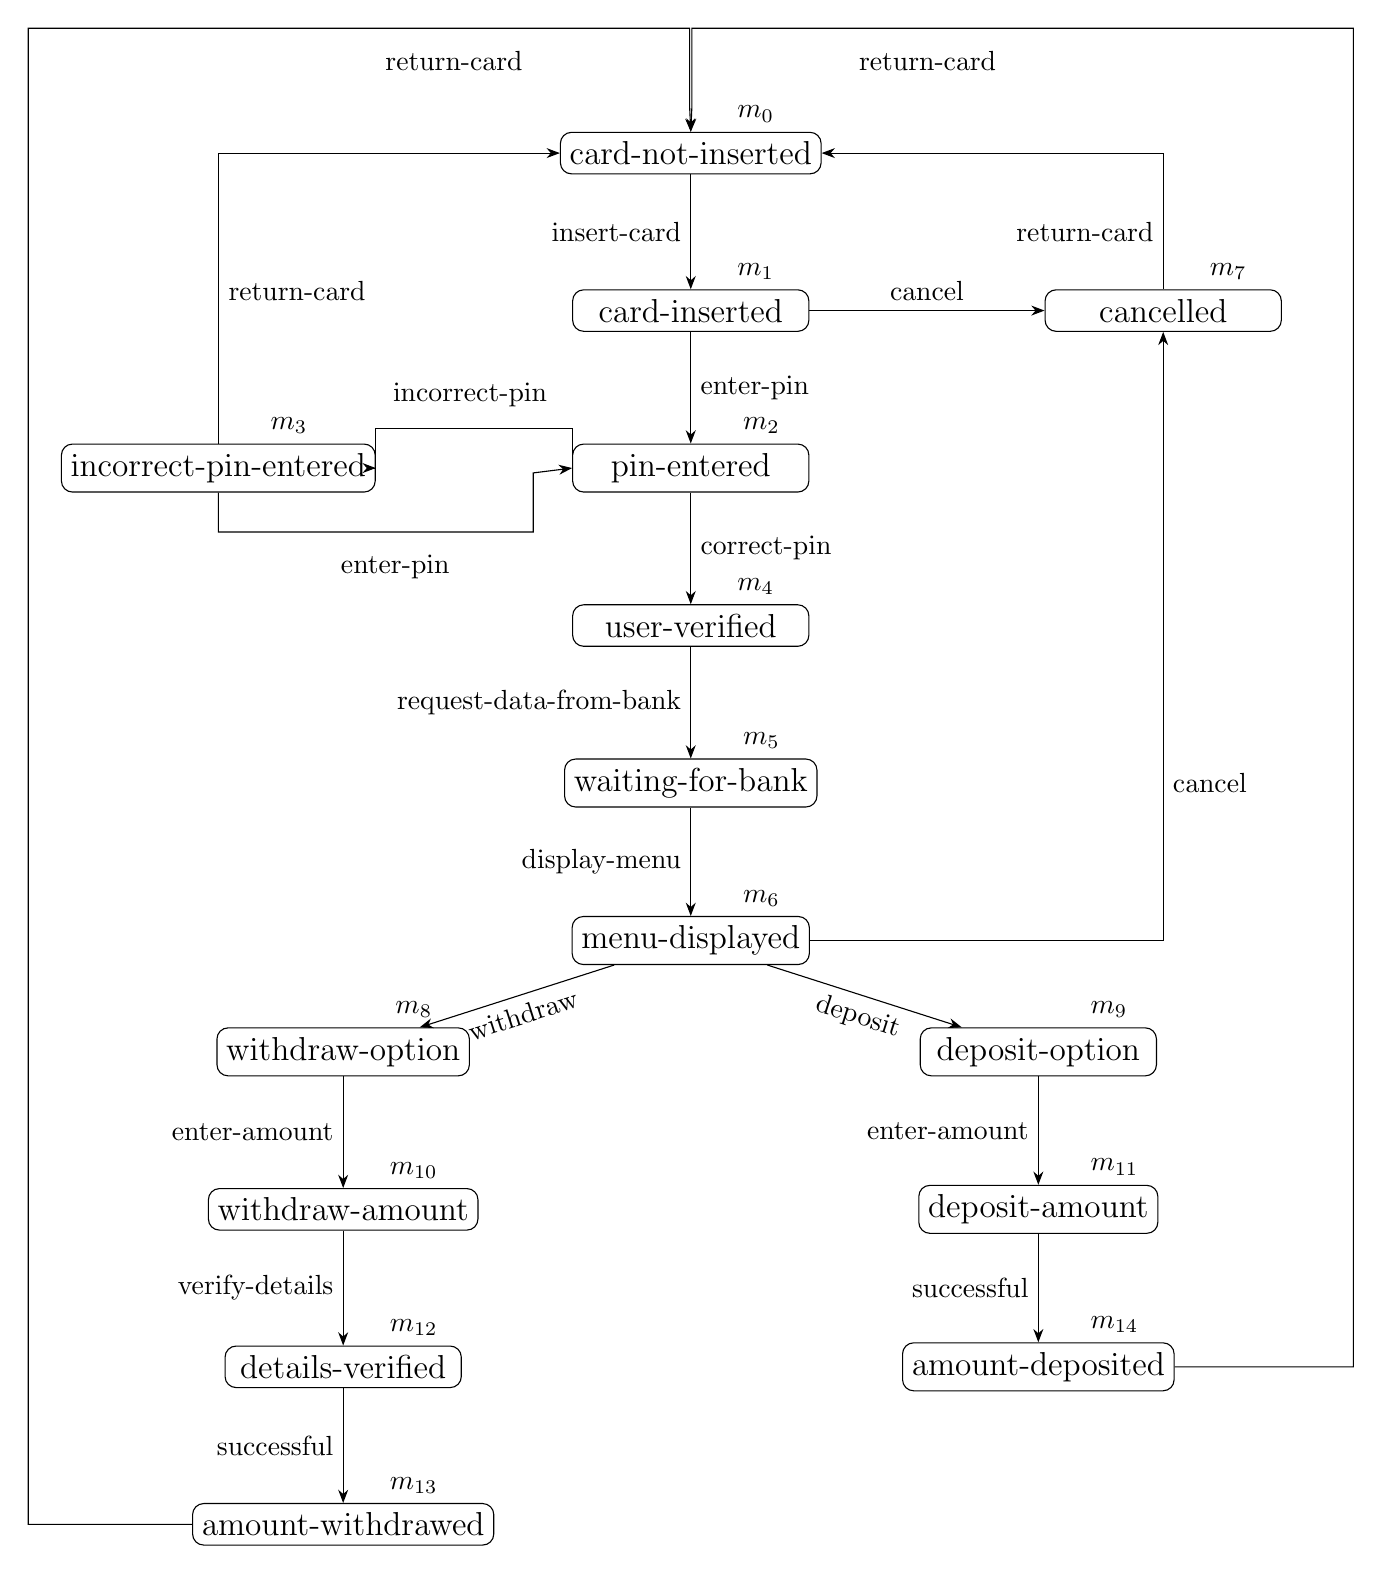
\begin{tikzpicture}[
			node distance=2cm,
			state/.style={rectangle, rounded corners, minimum width=3cm, minimum height=0.5cm,text centered, draw=black,font=\large},
			process/.style={rectangle, minimum width=3cm, minimum height=0.5cm, text centered, draw=black, fill=orange!30},
			io/.style={trapezium, trapezium left angle=70, trapezium right angle=110, minimum width=3cm, minimum height=1cm, text centered, draw=black, fill=blue!30},
			decision/.style={diamond, minimum width=3cm, minimum height=1cm, text centered, draw=black, fill=green!30},
			]
			
			\node[state]       (m_0) [label={[label]30:$m_0$}]                                        {card-not-inserted};
			\node[state]         (m_1) [below of=m_0, label={[label]30:$m_1$}]                          {card-inserted};
			\node[state]         (m_2) [below of=m_1, label={[label]30:$m_2$}]                          {pin-entered};
			\node[state]         (m_3) [left of=m_2, xshift=-4cm, label={[label]30:$m_3$}]              {incorrect-pin-entered};
			\node[state]         (m_4) [below of=m_2, label={[label]30:$m_4$}]                          {user-verified};
			\node[state]         (m_5) [below of=m_4, label={[label]30:$m_5$}]                          {waiting-for-bank};
			\node[state]         (m_6) [below of=m_5, label={[label]30:$m_6$}]                          {menu-displayed};
			\node[state]         (m_7) [right of=m_1, xshift=4cm, label={[label]30:$m_7$}]              {cancelled};
			\node[state]         (m_8) [below left of=m_6, xshift=-3cm, label={[label]30:$m_8$}]        {withdraw-option};
			\node[state]         (m_9) [below right of=m_6, xshift=3cm, label={[label]30:$m_9$}]        {deposit-option};
			\node[state]         (m_10) [below of=m_8, label={[label]30:$m_{10}$}]                      {withdraw-amount};
			\node[state]         (m_11) [below of=m_9, label={[label]30:$m_{11}$}]                      {deposit-amount};
			\node[state]         (m_12) [below of=m_10, label={[label]30:$m_{12}$}]                     {details-verified};
			\node[state]         (m_13) [below of=m_12, label={[label]30:$m_{13}$}]                     {amount-withdrawed};
			\node[state]         (m_14) [below of=m_11, label={[label]30:$m_{14}$}]                     {amount-deposited};
			
			
			\draw [arrows=-Stealth] (m_0)                                                    --node[anchor=east]                                              {insert-card}        (m_1);
			\draw [arrows=-Stealth] (m_1)                                                    --node[anchor=west]                                              {enter-pin}         (m_2);
			\draw [arrows=-Stealth] (m_1)                                                    --node[anchor=south]                                             {cancel}       (m_7);
			\draw [arrows=-Stealth] (m_2.west) -- ++(0,0.5)  -- ++(-2.5,0) -- ++(0,-0.5)     --node[xshift=1.2cm,yshift=1.2cm,anchor=north,below]             {incorrect-pin}       (m_3.east);
			\draw [arrows=-Stealth] (m_3.south) -- ++(0,-0.5) -- ++(4,0) -- ++(0,0.75)       --node[xshift=-2cm,yshift=-1.5cm,anchor=south]                   {enter-pin}    (m_2.west);
			\draw [arrows=-Stealth] (m_3)                                                    |-node[xshift=1cm,yshift=-1.5cm,anchor=north,below]              {return-card} (m_0);
			\draw [arrows=-Stealth] (m_2)                                                    --node[anchor=west]                                              {correct-pin}       (m_4);
			\draw [arrows=-Stealth] (m_4)                                                    --node[anchor=east]                                              {request-data-from-bank}(m_5);
			\draw [arrows=-Stealth] (m_5)                                                    --node[anchor=east]                                              {display-menu}         (m_6);
			\draw [arrows=-Stealth] (m_6)                                                    -|node[yshift=2cm,anchor=west]                                              {cancel}       (m_7);
			\draw [arrows=-Stealth] (m_7)                                                    |-node[yshift=-1cm,anchor=east]                                              {return-card}    (m_0);
			\draw [arrows=-Stealth] (m_6)                                                    --node[anchor=north,sloped]                                      {withdraw} (m_8);
			\draw [arrows=-Stealth] (m_6)                                                    --node[anchor=north,sloped]                                      {deposit}       (m_9);
			\draw [arrows=-Stealth] (m_8)                                                    --node[anchor=east]                                              {enter-amount}        (m_10);
			\draw [arrows=-Stealth] (m_10)                                                   --node[anchor=east]                                              {verify-details}   (m_12);
			\draw [arrows=-Stealth] (m_12)                                                   --node[anchor=east]                                              {successful}       (m_13);
			\draw [arrows=-Stealth] (m_13) -- ++(-4,0) -- ++(0,19) -- ++(8.4,0) -- ++(0,-1)              --node[xshift=-3cm,yshift=0.5cm,anchor=south]                     {return-card}    (m_0.north);
			\draw [arrows=-Stealth] (m_9)                                                    --node[anchor=east]                                              {enter-amount} (m_11);
			\draw [arrows=-Stealth] (m_11)                                                   --node[anchor=east]                                              {successful}       (m_14);
			\draw [arrows=-Stealth] (m_14) -- ++(4,0) -- ++(0,17) -- ++(-8.4,0) -- ++(0,-1)               -- node[xshift=3cm,yshift=0.5cm,anchor=south]                                            {return-card} (m_0.north);
			
			\end{tikzpicture}
		\end{adjustbox}
%			\caption{Mode graph of the ATM}
%			\label{fig:Mode graph of the ATM}
	\end{figure}
\end{frame}

\begin{frame}{Automated Teller Machine (ATM)}
	\begin{figure}
		\begin{adjustbox}{max totalsize={.99\textwidth}{.85\textheight},center}
		%	\begin{minipage}{.7\textwidth}
			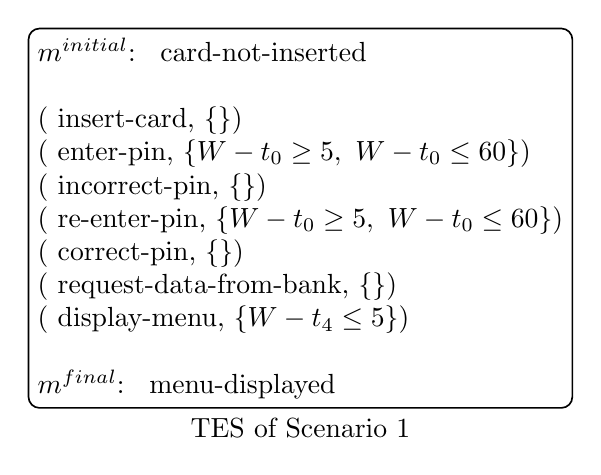
\begin{tikzpicture}[->,>=stealth']
			\tikzset{vertex/.style = {shape=rectangle,rounded corners, semithick, draw,align=left}}
			
			\node[vertex, label = below: TES of Scenario 1] (QUERY) 
			{ $m^{initial}$: { card-not-inserted} \\
				\\
				({ insert-card}, $\{\}$) \\
				({ enter-pin}, $\{W-t_0\geq 5,~W-t_0\leq 60\}$) \\
				({ incorrect-pin}, $\{\}$) \\
				({ re-enter-pin}, $\{W-t_0\geq 5,~W-t_0\leq 60\}$) \\
				({ correct-pin}, $\{\}$) \\
				({ request-data-from-bank}, $\{\}$) \\
				({ display-menu}, $\{W-t_4\leq 5\}$) \\
				\\
				$m^{final}$: { menu-displayed}
			};
			
			\end{tikzpicture}
		%\end{minipage}
		\hspace{0.5cm}
	%	\begin{minipage}{.7\textwidth}
			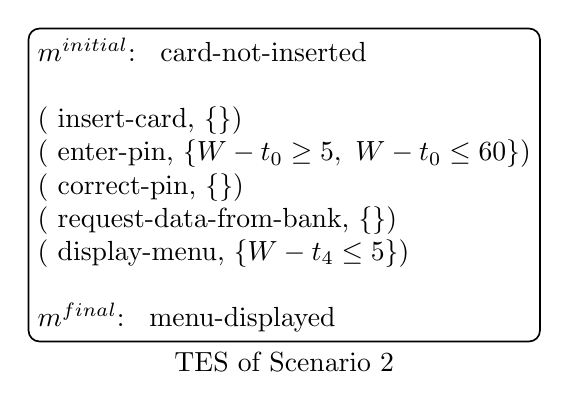
\begin{tikzpicture}[->,>=stealth']
			\tikzset{vertex/.style = {shape=rectangle,rounded corners, semithick, draw,align=left}}
			\node[vertex, label = below: TES of Scenario 2] (QUERY) 
			{ $m^{initial}$: { card-not-inserted} \\
				\\
				({ insert-card}, $\{\}$) \\
				({ enter-pin}, $\{W-t_0\geq 5,~W-t_0\leq 60\}$) \\
				({ correct-pin}, $\{\}$) \\
				({ request-data-from-bank}, $\{\}$) \\
				({ display-menu}, $\{W-t_4\leq 5\}$) \\
				\\
				$m^{final}$: { menu-displayed}
			};
			
			\end{tikzpicture}
	%	\end{minipage}
		\end{adjustbox}
		\caption{Timed Event Sequences of the ATM}
		\label{fig:Timed Event Sequences of ATM}
		
	\end{figure}
\end{frame}

\begin{frame}{Automated Teller Machine (ATM)}
	\begin{figure}
		\begin{adjustbox}{max totalsize={.99\textwidth}{.85\textheight},center}
		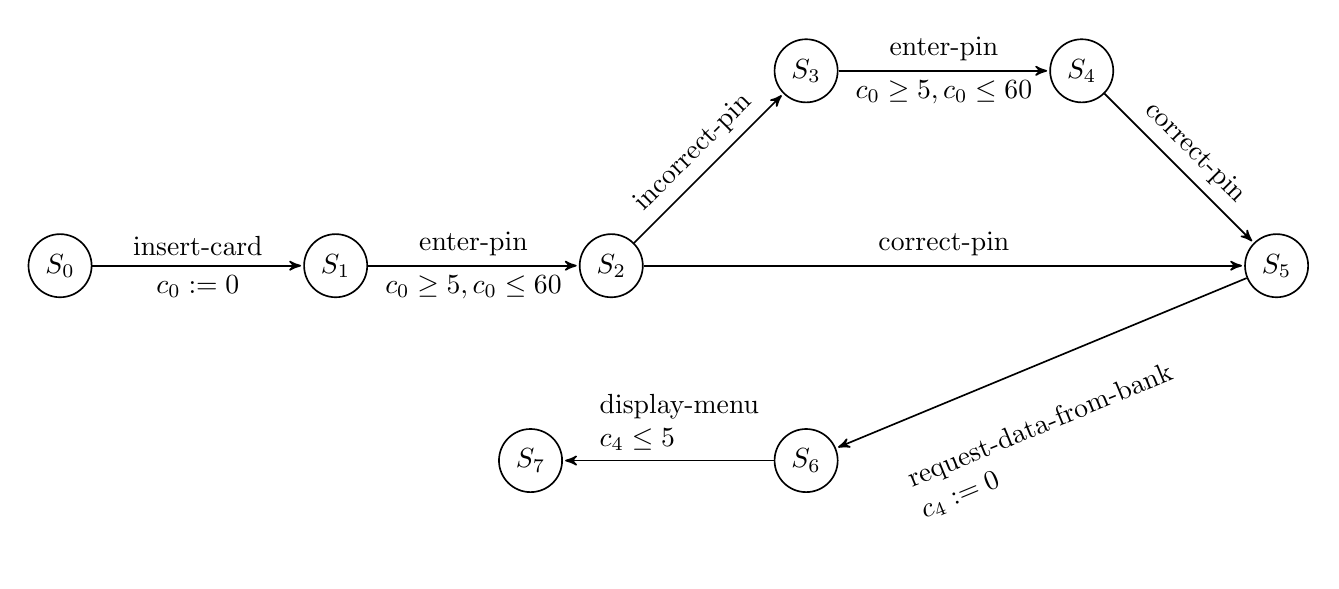
\begin{tikzpicture}[->,>=stealth',shorten >=0.8pt,auto,node distance=3.5cm,
		semithick]
		\tikzstyle{every state}=[draw,minimum size=1em]
		
		\node[state]         (S_0)              {$S_0$};
		\node[state]         (S_1) [right of=S_0] {$S_1$};
		\node[state]         (S_2) [right of=S_1] {$S_2$};
		\node[state]         (S_3) [above right of=S_2] {$S_3$};
		\node[state]         (S_4) [right of=S_3] {$S_4$};
		\node[state]         (S_5) [below right of=S_4] {$S_5$};
		\node[state]         (S_6) [below right of=S_2] {$S_6$};
		\node[state]         (S_7) [left of=S_6] {$S_7$}; 
		
		\path (S_0) edge                node[anchor=south, above]             {insert-card}           
		node[anchor=south, below]             {$c_0 := 0$}            (S_1)
		(S_1) edge                node[anchor=south, above]             {enter-pin} 
		node[anchor=north, below]             {$c_0\ge5,c_0\le60$}    (S_2)
		(S_2) edge                node[anchor=south, above,sloped]      {incorrect-pin}         (S_3)
		(S_3) edge                node[anchor=south, above]             {enter-pin} 
		node[anchor=north, below]             {$c_0\ge5,c_0\le60$}    (S_4)
		(S_4) edge                node[anchor=south, above,sloped]      {correct-pin}           (S_5)
		(S_2) edge                node[above]                           {correct-pin}           (S_5)
		(S_5) edge                node[anchor=north, below,sloped,text width=6cm]      {
			\centering
			\begin{itemize}
			\item[] request-data-from-bank\\$c_4 := 0$ 
			\end{itemize}
		}                       (S_6)
		(S_6) edge                node[anchor=south, above,text width=3.5cm] {
			\begin{itemize}
			\item[] display-menu\\$c_4\le5$
			\end{itemize}
		}                       (S_7)
		;
		\end{tikzpicture}
		\end{adjustbox}
		\caption{Timed automaton synthesized from Scenario 1 and Scenario 2}
		\label{fig:timedAutomaton}
	\end{figure}
\end{frame}

\begin{frame}{Automated Teller Machine (ATM)}
	Now consider an extended behaviour of the ATM machine. After the menu is displayed, assume that, the user can choose from the two available options:
	\vspace{0.5cm}
	\begin{columns}[T]
		\begin{column}{0.4\textwidth}
			\textbf{Deposit:}
			\begin{enumerate}
				\item User enters the amount to deposit, and
				\item ATM returns success message if the deposit is successful.
			\end{enumerate}
		\end{column}
		\begin{column}{0.51\textwidth}
			\textbf{Withdraw:}
			\begin{enumerate}
				\item User enters the amount to withdraw,
				\item Bank verifies the user details, and
				\item Returns success message if the withdraw is successful.
			\end{enumerate}
		\end{column}
	\end{columns}
\end{frame}

\begin{frame}{Automated Teller Machine (ATM)}
\begin{figure}
	\begin{adjustbox}{max totalsize={.99\textwidth}{.85\textheight},center}
		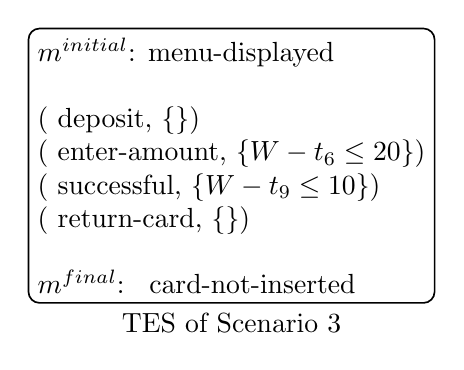
\begin{tikzpicture}[->,>=stealth']
		\tikzset{vertex/.style = {shape=rectangle,rounded corners, semithick, draw,align=left}}
		\node[vertex, label = below: TES of Scenario 3] (QUERY) 
		{ $m^{initial}$: {menu-displayed} \\
			\\
			({ deposit}, $\{\}$) \\
			({ enter-amount}, $\{W-t_6\leq 20\}$) \\
			({ successful}, $\{W-t_{9}\leq 10\}$) \\
			({ return-card}, $\{\}$) \\
			\\
			$m^{final}$: { card-not-inserted}
		};
		
		\end{tikzpicture}
	
		\hspace{0.5cm}
	
		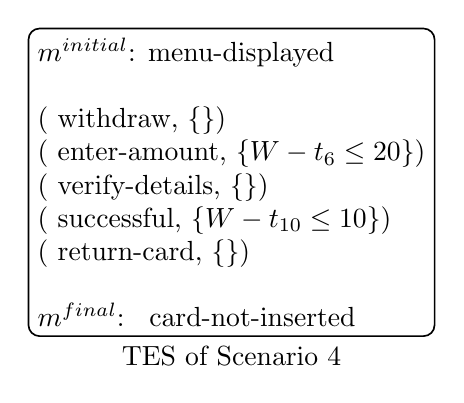
\begin{tikzpicture}[->,>=stealth']
		\tikzset{vertex/.style = {shape=rectangle,rounded corners, semithick, draw,align=left}}
		\node[vertex, label = below: TES of Scenario 4] (QUERY) 
		{ $m^{initial}$: {menu-displayed} \\
			\\
			({ withdraw}, $\{\}$) \\
			({ enter-amount}, $\{W-t_6\leq 20\}$) \\
			({ verify-details}, $\{\}$) \\
			({ successful}, $\{W-t_{10}\leq 10\}$) \\
			({ return-card}, $\{\}$) \\
			\\
			$m^{final}$: { card-not-inserted}
		};
		
		\end{tikzpicture}
		\end{adjustbox}
		\caption{Timed Event Sequences of the ATM with withdraw and deposit option}
		\label{fig:Timed Event Sequences of ATM with withdraw and deposit option}
	\end{figure}

\end{frame}

\begin{frame}{Automated Teller Machine (ATM)}
	\begin{figure}
		\begin{adjustbox}{max totalsize={.99\textwidth}{.85\textheight},center}			
			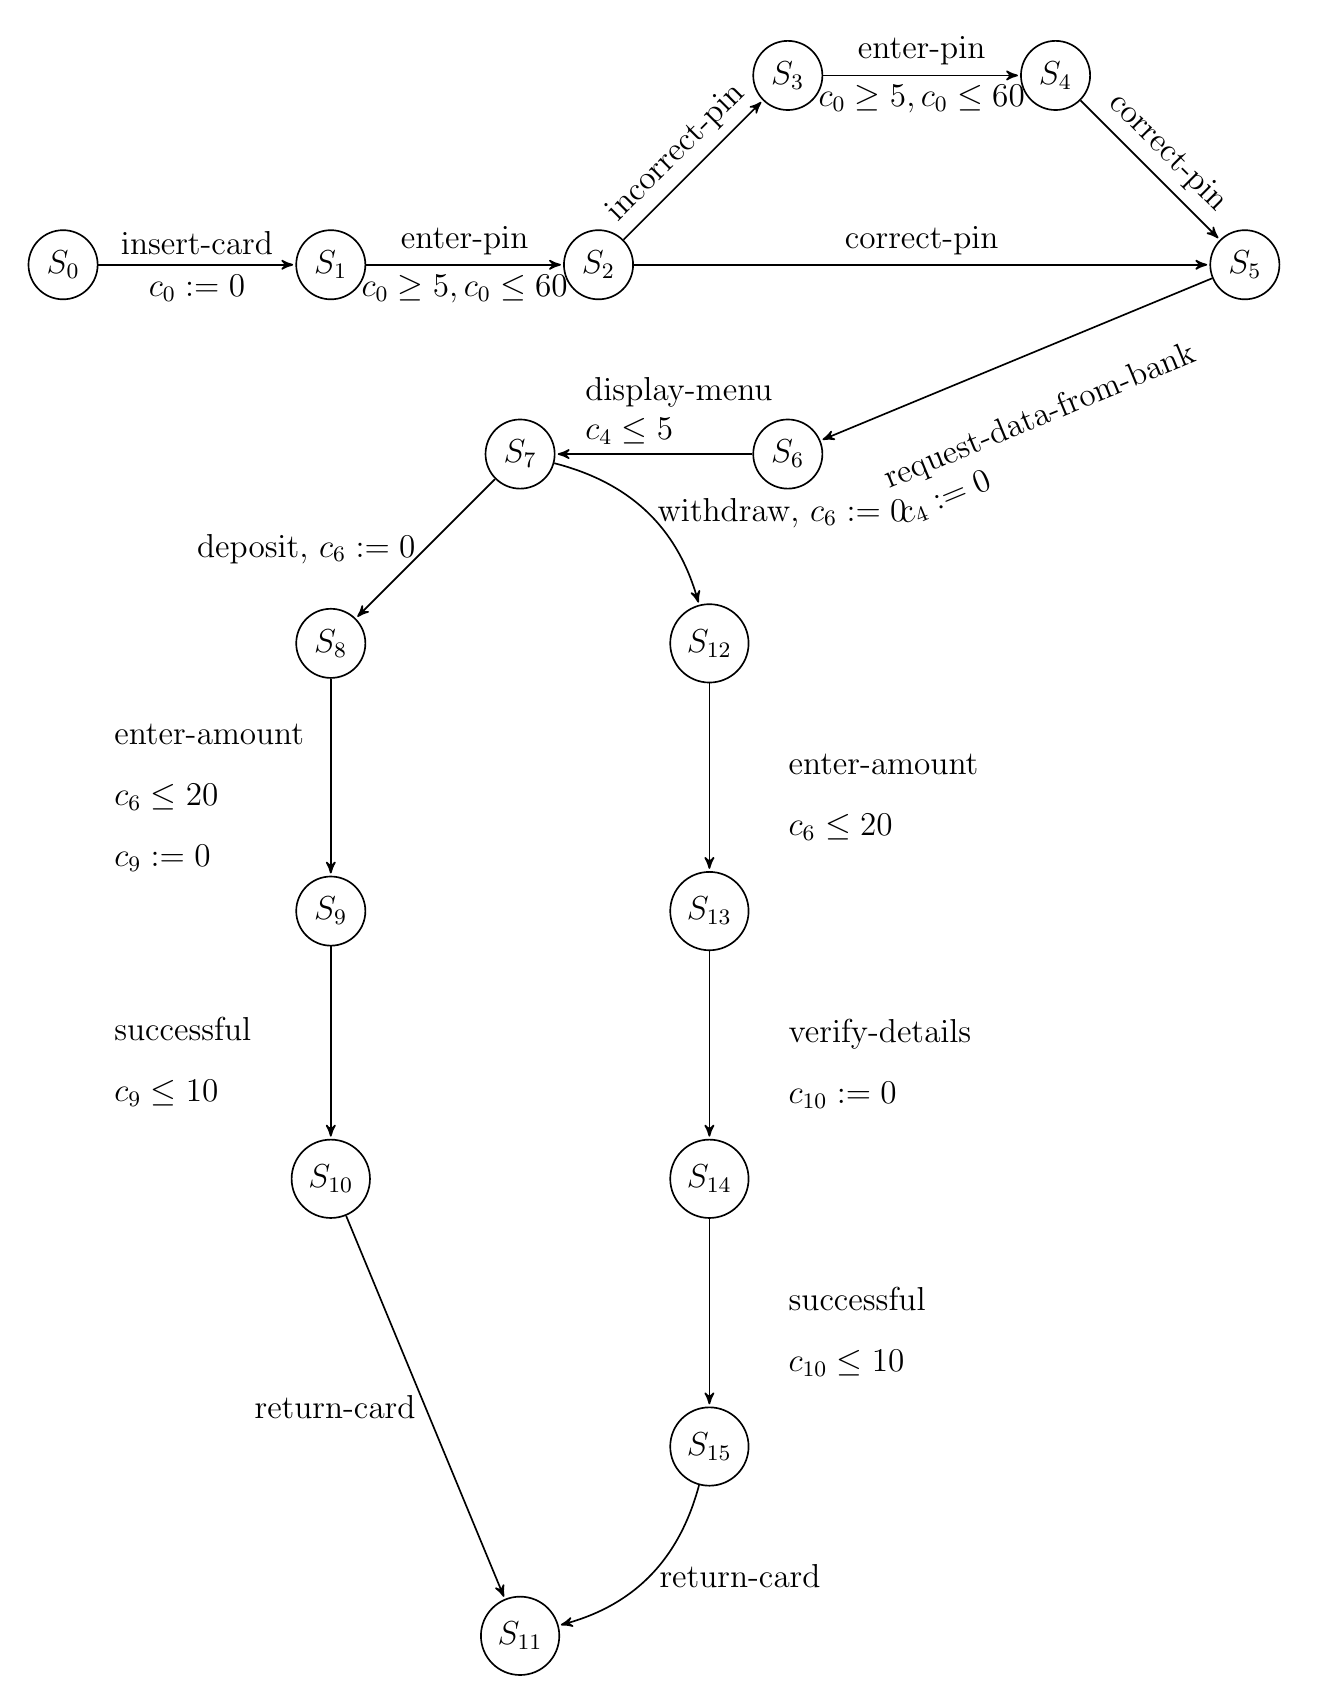
\begin{tikzpicture}[->,>=stealth',shorten >=0.8pt,auto,node distance=3.4cm,
			semithick,font=\large]
			\tikzstyle{every state}=[draw,minimum size=1em]
			
			\node[state]         (S_0)              {$S_0$};
			\node[state]         (S_1) [right of=S_0] {$S_1$};
			\node[state]         (S_2) [right of=S_1] {$S_2$};
			\node[state]         (S_3) [above right of=S_2] {$S_3$};
			\node[state]         (S_4) [right of=S_3] {$S_4$};
			\node[state]         (S_5) [below right of=S_4] {$S_5$};
			\node[state]         (S_6) [below right of=S_2] {$S_6$};
			\node[state]         (S_7) [left of=S_6] {$S_7$};
			\node[state]         (S_8) [below left of=S_7] {$S_8$};
			
			\node[state]         (S_9) [below of=S_8] {$S_9$};
			\node[state]         (S_10) [below of=S_9] {$S_{10}$};
			
			\node[state]         (S_12) [below right of=S_7] {$S_{12}$};
			\node[state]         (S_13) [below of=S_12] {$S_{13}$};
			\node[state]         (S_14) [below of=S_13] {$S_{14}$};
			\node[state]         (S_15) [below of=S_14] {$S_{15}$};
			\node[state]         (S_11) [below left of=S_15] {$S_{11}$};
			
						
			\path (S_0) edge                node[anchor=south, above]             {insert-card}           
			node[anchor=south, below]             {$c_0 := 0$}            (S_1)
			(S_1) edge                node[anchor=south, above]             {enter-pin} 
			node[anchor=north, below]             {$c_0\ge5,c_0\le60$}    (S_2)
			(S_2) edge                node[anchor=south, above,sloped]      {incorrect-pin}         (S_3)
			(S_3) edge                node[anchor=south, above]             {enter-pin} 
			node[anchor=north, below]             {$c_0\ge5,c_0\le60$}    (S_4)
			(S_4) edge                node[anchor=south, above,sloped]      {correct-pin}           (S_5)
			(S_2) edge                node[above]                           {correct-pin}           (S_5)
			(S_5) edge                node[anchor=north, below,sloped,text width=6cm]      {
				\centering
				\begin{itemize}
				\item[] request-data-from-bank\\$c_4 := 0$ 
				\end{itemize}
			}                       (S_6)
			(S_6) edge                node[anchor=south, above,text width=3.5cm] 
			{ 
				\begin{itemize}
				\item[] display-menu\\$c_4\le5$
				\end{itemize}
			}                       (S_7)
			(S_7) edge                node[left]                            {deposit, $c_6:=0$}               (S_8)
			
			(S_8) edge                node[anchor=right, left,text width=3.5cm] 
			{ 
				\begin{itemize}
				\item[] enter-amount
				\item[] $c_6\le20$
				\item[] $c_9:=0$
				\end{itemize}
			}                        (S_9)
			(S_9) edge                node[anchor=right, left,text width=3.5cm] 
			{ 
				\begin{itemize}
				\item[] successful
				\item[] $c_{9}\le10$
				\end{itemize}
			}                       (S_10)
			(S_10) edge               node[left]                            {return-card}           (S_11)
			
			(S_7) edge   [bend left]  node[right]                           {withdraw, $c_6:=0$}              (S_12)
			(S_12) edge               node[anchor=left, right,text width=3.5cm] 
			{ 
				\begin{itemize}
				\item[] enter-amount
				\item[] $c_6\le20$
				\end{itemize}
			}                       (S_13)
			(S_13) edge               node[anchor=left, right,text width=3.5cm] 
			{ 
				\begin{itemize}
				\item[] verify-details
				\item[] $c_{10}:= 0$
				\end{itemize}
			}                       (S_14)
			(S_14) edge               node[anchor=left, right,text width=3.5cm] 
			{ 
				\begin{itemize}
				\item[] successful
				\item[] $c_{10}\le10$
				\end{itemize}
			}                       (S_15)
			(S_15) edge  [bend left]  node[right]                           {return-card}           (S_11)
			;
			\end{tikzpicture}
		\end{adjustbox}
		\caption{The synthesized timed automaton of the ATM}
		\label{fig:Synthesized ATM TA}
	\end{figure}
\end{frame}


\begin{frame}{Light Control System}
	Consider the variant of the light control system:
	\begin{enumerate}
		\item $Idle$ is both the initial and final mode ,
		\item The mode changes from $Idle$ to $Light$ upon issuing the command $ON$, and
		\item If $ON$ is issued again within 3 units of time, the light will go $Bright$. Else the light goes back to $Idle$. 
	\end{enumerate}
	
	\begin{figure}[!ht]
		\begin{adjustbox}{max totalsize={.80\textwidth}{.80\textheight},center}
%			\begin{minipage}{0.8\textwidth}
				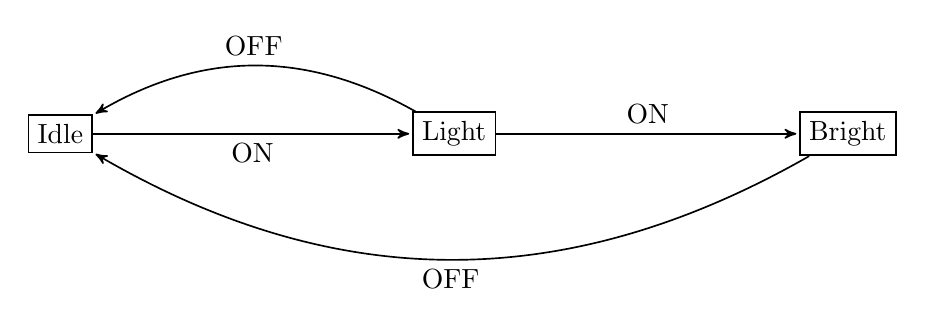
\begin{tikzpicture}[->,>=stealth',shorten >=1pt,auto,node distance=5cm,
				semithick]
				\tikzstyle{every state}=[shape=rectangle,draw,minimum size=1em]
				
				\node[state]       (Idle)                    {Idle};
				\node[state]       (Light)  [right of=Idle]     {Light};
				\node[state]       (Bright) [right of=Light]     {Bright};
				
				\path (Idle) edge                   node[below]  {ON}  (Light)
				(Light) edge    [bend right]  node[above]  {OFF}  (Idle)
				(Light) edge                  node[above]  {ON}  (Bright)
				(Bright) edge   [bend left]   node[below]  {OFF}  (Idle)    
				;
				\end{tikzpicture}
%			\end{minipage}
		\end{adjustbox}
		\caption{Mode graph of the Light Control System}
		\label{fig:MG_Light Control System}
	\end{figure}
\end{frame}

\begin{frame}{Light Control System}
		\begin{figure}
			\begin{adjustbox}{max totalsize={.99\textwidth}{.85\textheight},center}
	
%			\begin{minipage}[b]{.25\textwidth}
				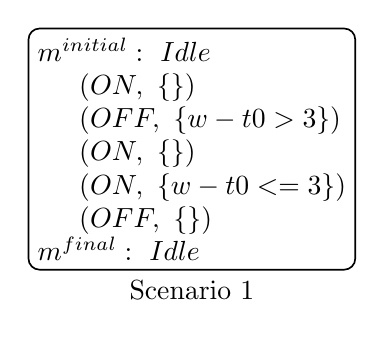
\begin{tikzpicture}[->,>=stealth']
				\tikzset{vertex/.style = {shape=rectangle,rounded corners, semithick, draw,align=left}}
				\node[vertex, label = below: Scenario 1] (QUERY) 
				{$m^{initial}:~Idle$ \\                                
					\indent    ($ON,~\{\}$) \\
					\indent    ($OFF, ~\{w-t0 > 3\}$) \\
					\indent    ($ON,~\{\}$) \\
					\indent    ($ON, ~\{w-t0 <= 3\}$) \\
					\indent    ($OFF,~\{\}$) \\                
					$m^{final}:~Idle$};
				
				\end{tikzpicture}
%			\end{minipage}
			\hspace{0.5cm}
%			\begin{minipage}[b]{.25\textwidth}
				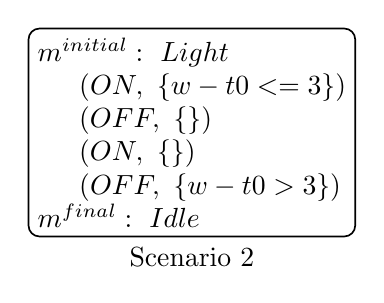
\begin{tikzpicture}[->,>=stealth']
				\tikzset{vertex/.style = {shape=rectangle,rounded corners, semithick, draw,align=left}}
				\node[vertex, label = below: Scenario 2] (QUERY) 
				{$m^{initial}:~Light$ \\
					
					\indent    ($ON,~\{w-t0 <= 3\}$) \\
					\indent    ($OFF,~\{\}$) \\
					\indent    ($ON,~\{\}$) \\
					\indent    ($OFF,~\{w-t0 > 3\}$) \\
					
					$m^{final}:~Idle$};
				
				\end{tikzpicture}
%			\end{minipage}
			\hspace{0.5cm}
%			\begin{minipage}[b]{.25\textwidth}
				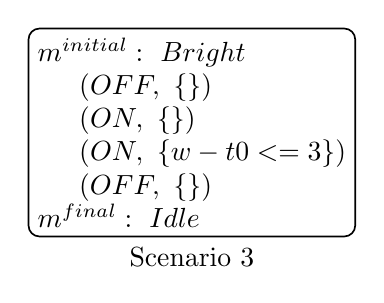
\begin{tikzpicture}[->,>=stealth']
				\tikzset{vertex/.style = {shape=rectangle,rounded corners, semithick, draw,align=left}}
				\node[vertex, label = below: Scenario 3] (QUERY) 
				{$m^{initial}:~Bright$ \\
					
					\indent    ($OFF,~\{\}$) \\
					\indent    ($ON,~\{\}$) \\
					\indent    ($ON,~\{w-t0 <= 3\}$) \\
					\indent    ($OFF,~\{\}$) \\
					
					$m^{final}:~Idle$};
				
				\end{tikzpicture}
%			\end{minipage}
		
		\end{adjustbox}
		\caption{Timed Event Sequences of the Light Control System}
		\label{fig:Timed Event Sequences of Light Control System}
	\end{figure}
\end{frame}

\begin{frame}{Light Control System}
	\begin{figure}
		\begin{adjustbox}{max totalsize={.99\textwidth}{.8\textheight},center}
			\begin{tikzpicture}[->,>=stealth',shorten >=1pt,auto,node distance=2.3cm,
			semithick]
			\tikzstyle{every state}=[draw,minimum size=1.65cm]
			
			\node[state]         (S_0) [yshift=-1.5cm]                   {$Idle$};
			\node[state]         (S_1) [below of=S_0,yshift=-1cm]     {$Light$};
			\node[state]         (S_2) [below of=S_1,yshift=-1cm]     {$Idle$};
			\node[state]         (S_3) [below of=S_2,yshift=-1cm]     {$Light$};
			\node[state]         (S_4) [below of=S_3,yshift=-1cm]   {$Bright$};
			\node[state]         (S_5) [right of=S_4,xshift=1cm]    {$Idle$};
			\node[state]         (S_6) [right of=S_5,xshift=1.6cm]    {$Light$};
			\node[state]         (S_7) [right of=S_6,xshift=1.6cm]    {$Idle$};
			\node[state]         (S_8) [above right of=S_6,xshift=1cm,yshift=1cm]    {$Bright$};
			
			\path (S_0) edge              node[right]  {ON [$c_0 := 0$]}  (S_1)
			(S_1) edge              node[right]  {OFF [$c_0 > 3$]}  (S_2)
			(S_2) edge              node[right]  {ON [$c_0 := 0$]}  (S_3)
			(S_1) edge [bend right] node[left]   {ON [$c_0 <= 3$]}  (S_4)
			(S_3) edge              node[right]  {ON [$c_0 <= 3$]}  (S_4)
			(S_4) edge              node[below]  {OFF}  (S_5)
			(S_5) edge              node[below]  {ON [$c_0 := 0$]}  (S_6)
			(S_6) edge              node[below]  {OFF [$c_0 > 3$]}  (S_7)
			(S_6) edge [bend left]  node[left]   {ON [$c_0 <= 3$]}  (S_8)
			(S_8) edge [bend left]  node[right]  {OFF}  (S_7)
			
			;
			\end{tikzpicture}
		\end{adjustbox}
	
		\caption{Timed automaton of the Light Control System}
		\label{fig:TA_Ligt Control System}
	\end{figure}
\end{frame}

\begin{frame}{Traffic Light}
Consider the behaviour of a traffic light. 
	\begin{itemize}
		\item {The system periodically moves from $Initial \rightarrow Red$, $Red \rightarrow Yellow$, $yellow \rightarrow Green$, and then it is $Reset$},
		\item {On the transitions $turn-yellow$ and $turn-green$ a clock constraint is checked and a new clock is born.}
	\end{itemize}
	\vspace{0.2cm}
	\begin{figure}
		\begin{adjustbox}{max totalsize={.99\textwidth}{.8\textheight},center}
		
		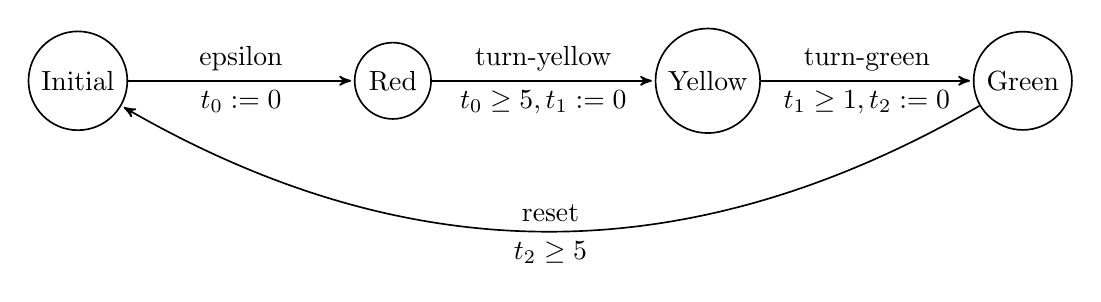
\begin{tikzpicture}[->,>=stealth',shorten >=1pt,auto,node distance=4cm,
		semithick]
		\tikzstyle{every state}=[draw,minimum size=1em]
		
		\node[state]       (Initial)                        {Initial};
		\node[state]       (Red)      [right of=Initial]    {Red};
		\node[state]       (Yellow)   [right of=Red]        {Yellow};
		\node[state]       (Green)    [right of=Yellow]      {Green};
		
		
		\path (Initial)   edge          node[anchor=south, above] {epsilon} 
		node[anchor=north, below] {$t_0:=0$}       (Red)
		(Red)       edge                 node[anchor=south, above] {turn-yellow}
		node[anchor=north, below] {$t_0\ge5,t_1:=0$}     (Yellow)
		(Yellow)    edge                 node[anchor=south, above] {turn-green} 
		node[anchor=north, below] {$t_1\ge1,t_2:=0$}     (Green)
		(Green)     edge   [bend left]   node[anchor=south, above] {reset} 
		node[anchor=north, below] {$t_2\ge5$}           (Initial)   
		;
		\end{tikzpicture}
		\end{adjustbox}
		\caption{Timed automaton of the Traffic Light}
		\label{fig:TrafficLight}		
	\end{figure}
\end{frame}

\begin{frame}{Traffic Light}
	\begin{figure}
		\begin{adjustbox}{max totalsize={.99\textwidth}{.8\textheight},center}		
	
		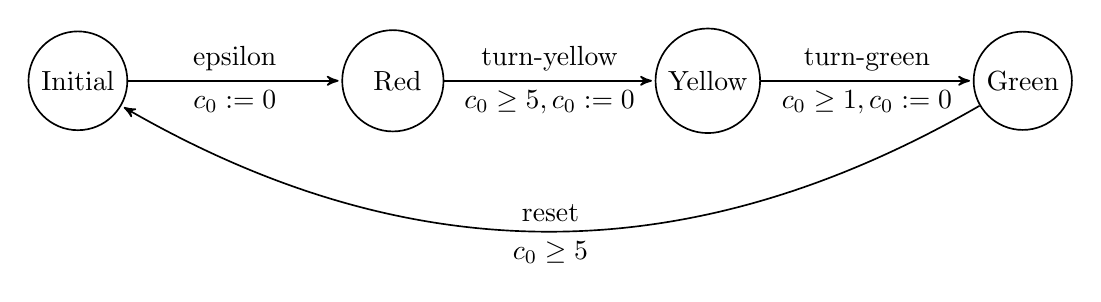
\begin{tikzpicture}[->,>=stealth',shorten >=1pt,auto,node distance=4cm,
		semithick]
		\tikzstyle{every state}=[draw,minimum size=1em]
		
		\node[state]       (Initial)                        {Initial};
		\node[state]       (Red)      [right of=Initial]    {~~Red~~};
		\node[state]       (Yellow)   [right of=Red]        {Yellow};
		\node[state]       (Green)    [right of=Yellow]      {Green};
		
		
		\path (Initial)   edge          node[anchor=south, above] {epsilon} 
		node[anchor=north, below] {$c_0:=0$}       (Red)
		(Red)       edge                 node[anchor=south, above] {turn-yellow}
		node[anchor=north, below] {$c_0\ge5,c_0:=0$}     (Yellow)
		(Yellow)    edge                 node[anchor=south, above] {turn-green} 
		node[anchor=north, below] {$c_0\ge1,c_0:=0$}     (Green)
		(Green)     edge   [bend left]   node[anchor=south, above] {reset} 
		node[anchor=north, below] {$c_0\ge5$}           (Initial)   
		;
		\end{tikzpicture}
	
		\end{adjustbox}
		\caption{The optimally allocated timed automaton of the Traffic Light}
		\label{fig:OptimalTrafficLight}
	\end{figure}
\end{frame}

\begin{frame}{CSMA/CD Protocol}
	Consider a variant of the CSMA/CD protocol.
	\begin{figure}
		\begin{adjustbox}{max totalsize={.99\textwidth}{.75\textheight},center}	
			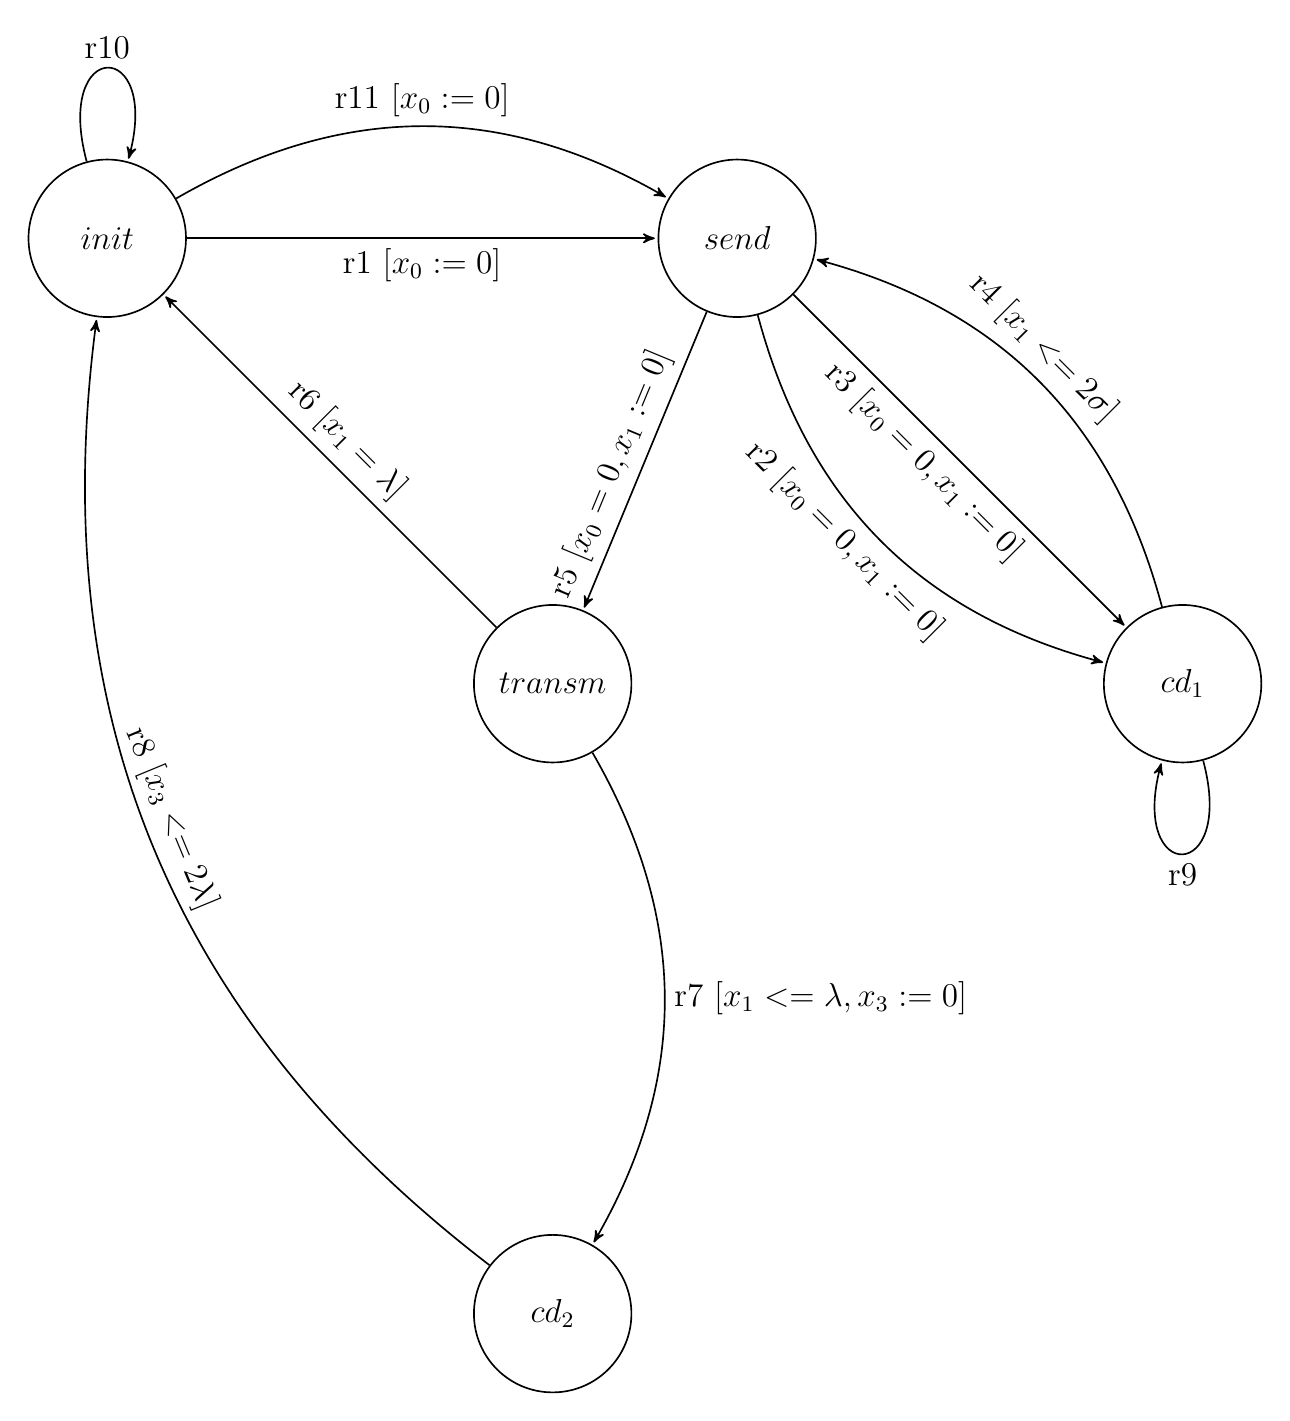
\begin{tikzpicture}[->,>=stealth',shorten >=1pt,auto,node distance=8cm,
			semithick,font=\large]
			\tikzstyle{every state}=[draw,minimum size=2cm]
			
			\node[state]         (init)                    {$init$};
			\node[state]         (send) [right of=init]  {$send$};
			\node[state]         (cd_1) [below right of=send]  {$cd_1$};
			\node[state]         (transm) [left of=cd_1] {$transm$};
			\node[state]         (cd_2) [below of=transm]  {$cd_2$};
			
			
			\path (init) edge                   node[below] {r1  [$x_0:=0$]}  (send)
			(init) edge   [bend left]     node[above] {r11 [$x_0:=0$]}  (send)
			(init) edge   [loop above]    node[]      {r10}  (init)
			(send) edge   [bend right]    node[sloped,anchor=center,below,text width=4cm]  {r2  [$x_0=0,x_1:=0$]}  (cd_1)
			(send) edge                   node[sloped,anchor=center,below,text width=4cm]  {r3  [$x_0=0,x_1:=0$]}  (cd_1)
			(send) edge                   node[sloped,anchor=center,above,text width=4cm]  {r5  [$x_0=0,x_1:=0$]}  (transm)
			(cd_1) edge   [bend right]    node[sloped,anchor=center,above,text width=3cm] {r4  [$x_1<=2\sigma$]}  (send)
			(cd_1) edge   [loop below]    node[]      {r9}  (cd_1)
			(transm) edge                 node[sloped,anchor=center,above,text width=2cm]  {r6  [$x_1=\lambda$]}  (init)
			(transm) edge [bend left]     node[right]  {r7  [$x_1<=\lambda,x_3:=0$]}  (cd_2)
			(cd_2) edge   [bend  left]    node[sloped,anchor=center,above,text width=3cm]  {r8  [$x_3<=2\lambda$]}  (init)
			
			;
			\end{tikzpicture}
		\end{adjustbox}
		\caption{The timed automaton for the sender in CSMA/CD protocol}
		\label{fig:CSMA/CD}
	\end{figure}
\end{frame}


\begin{frame}{CSMA/CD Protocol}
	\begin{figure}
		\begin{adjustbox}{max totalsize={.99\textwidth}{.8\textheight},center}	

		\begin{tikzpicture}[->,>=stealth',shorten >=1pt,auto,node distance=8cm,
		semithick,font=\large]
		\tikzstyle{every state}=[draw,minimum size=2cm]
		
		\node[state]         (init)                    {$init$};
		\node[state]         (send) [right of=init]  {$send$};
		\node[state]         (cd_1) [below right of=send]  {$cd_1$};
		\node[state]         (transm) [left of=cd_1] {$transm$};
		\node[state]         (cd_2) [below of=transm]  {$cd_2$};
		
		
		\path (init) edge                   node[below]                                      {r1  [$c_1:=0$]}  (send)
		(init) edge   [bend left]     node[above]                                      {r11 [$c_1:=0$]}  (send)
		(init) edge   [loop above]    node[]                                           {r10}             (init)
		(send) edge   [bend right]    node[sloped,anchor=center,below,text width=4cm]  {r2  [$c_1=0,c_2:=0$]}  (cd_1)
		(send) edge                   node[sloped,anchor=center,below,text width=4cm]  {r3  [$c_1=0,c_2:=0$]}  (cd_1)
		(send) edge                   node[sloped,anchor=center,above,text width=4cm]  {r5  [$c_1=0,c_2:=0$]}  (transm)
		(cd_1) edge   [bend right]    node[sloped,anchor=center,above,text width=3cm]  {r4  [$c_2<=2\sigma$]}  (send)
		(cd_1) edge   [loop below]    node[]                                           {r9}                    (cd_1)
		(transm) edge                 node[sloped,anchor=center,above,text width=2cm]  {r6  [$c_1=\lambda$]}  (init)
		(transm) edge [bend left]     node[right]                                      {r7  [$c_1<=\lambda,c_1:=0$]}  (cd_2)
		(cd_2) edge   [bend  left]    node[sloped,anchor=center,above,text width=3cm]  {r8  [$c_1<=2\lambda$]}  (init)
		
		;
		\end{tikzpicture}
		\end{adjustbox}
		\caption{The optimally allocated timed automaton for the sender in CSMA/CD protocol}
		\label{fig:OptimalCSMA/CD}
	\end{figure}
\end{frame}

\section{Conclusion}

\begin{frame}{Conclusion}
	\begin{itemize}
		\item Proposed Timed Event Sequences to formally represent scenarios,
		%\pause
		\item Developed and implemented an algorithm to construct timed automaton  from a given set of scenarios expressed as TES and a mode graph,
		%\pause
		\item The synthesized timed automaton is minimal, deterministic and acyclic,
		%\pause
		\item The generated timed automaton belongs to a class of timed automata that satisfies the dominance assumption,
		%\pause
		\item Developed and implemented an optimal clock allocation algorithm to a class of timed automata that satisfies the dominance assumption, and
		%\pause
		\item Our algorithm, does not change the size of the original timed automaton and its complexity is quadratic in the size of the graph.
	\end{itemize}
\end{frame}

\begin{frame}[standout]
\Huge THANK YOU! \\
\vspace{0.5cm}
\small

\emph{Dr. Neda Saeedloei}\\
\emph{Dr. Henry Wang}\\
\emph{Dr. Ping Zhao}\\
\emph{all the faculty members and students.}
\end{frame}

\begin{frame}[standout]
	Questions?
\end{frame}


\begin{frame}[allowframebreaks]{References}
	\bibliography{ResearchPPT}
	\bibliographystyle{abbrv}
\end{frame}

\end{document}